%-------------------- begin preamble ----------------------

\documentclass
[twocolumn,
secnumarabic,
nobibnotes,
aps,
prl,
reprint,
groupedaddress,
amsmath,
amssymb,
]{revtex4-2}
\usepackage[caption=false]{subfig}
\usepackage{relsize,makeidx,color,setspace,amsfonts}
\usepackage{mathtools}


\usepackage{listings}
\lstset{
    language=Python,
    inputencoding=utf8,
    extendedchars=true,
    literate={ø}{{\o}}1 {å}{{\r a}}1 {Å}{{\r A}}1 {æ}{{\ae}}1,
    backgroundcolor=\color{white},
    basicstyle=\footnotesize\ttfamily,
    breakatwhitespace=false,
    breaklines=true,
    captionpos=b,
    commentstyle=\itshape\color{purple!60!black},
    frame=single,
    %identifierstyle=\color{orange},
    keepspaces=true,
    keywordstyle=\bfseries\color{violet},
    numbers=left,
    numbersep=5pt,
    numberstyle=\tiny\color{black},
    rulecolor=\color{black},
    showstringspaces=false,
    showtabs=false,
    stepnumber=1,
    stringstyle=\color{purple!60!black},
    tabsize=2,
    title=\lstname
  }
\usepackage{dcolumn}% Align table columns on decimal point
% \usepackage[table]{xcolor}
\usepackage[table,xcdraw]{xcolor}
% \usepackage[table,xcdraw]{xcolor}
\usepackage{bm,ltablex,microtype}
\usepackage{longtable}
\usepackage{siunitx}
\usepackage{algorithm2e}
\usepackage{csvsimple}
\usepackage{url}
\renewcommand{\UrlFont}{\small\tt}

\usepackage[pdftex]{graphicx}

\usepackage{fancyvrb} % packages needed for verbatim environments

\usepackage[T1]{fontenc}

\usepackage{ucs}
\usepackage[utf8]{inputenc}

\usepackage{neuralnetwork}

\usepackage{lmodern}         % Latin Modern fonts derived from Computer Modern

\usepackage{tikz}



% Hyperlinks in PDF:
\definecolor{linkcolor}{rgb}{0,0,0}
\definecolor{urlcolor}{rgb}{0,0,1}
\usepackage{hyperref}
\hypersetup{
breaklinks=true,
colorlinks=true,
linkcolor=linkcolor,
urlcolor=urlcolor,
citecolor=black,
filecolor=black,
%filecolor=blue,
pdfmenubar=true,
pdftoolbar=true,
bookmarksdepth=3   % Uncomment (and tweak) for PDF bookmarks with more levels than the TOC
}

\usepackage{csvsimple}
\usepackage{todonotes}
\setcounter{tocdepth}{2}  % levels in table of contents

% prevent orhpans and widows
\clubpenalty = 10000
\widowpenalty = 10000

% --- end of standard preamble for documents ---

% insert custom LaTeX commands...

\raggedbottom
\makeindex
\setlength{\textheight}{9.5in}


%-------------------- end preamble ----------------------

\begin{document}

% ------------------- main content ----------------------

\title{Time series forecasting using LSTMs \\ Project 3 - FYS-STK4155}
\author{David Andreas Bordvik}
\email{davidabo@mail.uio.no}
\affiliation{Department of Informatics, University of Oslo}
\author{Gard Pavels Høivang}
\email{gardph@mail.uio.no}
\author{Are Frode Kvanum}
\email{afkvanum@mail.uio.no}
\affiliation{Department of Geoscience, University of Oslo}

\date{\today}

\begin{abstract}
  \begin{description}
  \item[Background] This part would describe the
  context needed to understand what the paper
  is about.
  \item[Purpose] This part would state the purpose
  of the present paper.
  \item[Method] This part describe the methods
  used in the paper.
  \item[Results] This part would summarize the
  results.
  \item[Conclusions] This part would state the
  conclusions of the paper.
  \end{description}
\end{abstract}

\maketitle

\section{Introduction}
The Norwegian and European power markets are changing. Several trends and demands in todays society result in increased electricity usage and power consumption. Additionally, a higher integrated fraction of renewable energy production coupled with tighter integration of power transmission infrastructure between countries affects several aspects within the power market, such as; electricity price, electricity production, electricity transmission, and electricity demand. A tighter connection of power infrastructure between countries also connects the power markets between countries to a greater extend, giving room for a growing number of market participants and competition. In the light of increased market coupling, a higher fraction of renewable energy production, and increasingly competitive power markets, the need for forecasting the electricity price has become a fundamental process for energy companies. The ability to make qualitative decisions through forecasting the electricity price has never been more relevant. \cite{nowotarski_recent_2018}. Considering the aforementioned, studying what drives the power markets and the electricity price in the light of the current extreme prices motivates to this project. The extreme electricity price does not just affect the consumers of household electricity, it affects the society as a whole. To study the complex problem of electricity price forecasing, it was required for this project to tackle many different aspects such as: Studying of mechanisms of the power market, data collection trough API, data-preprocessing, time-series problem analysis, advanced time-series forecasting using both classical and neural network. For the forecasting part of this project, we settled on forecasting the electricity price for the next day at an hourly resolution (24 hours). The forecasting time-span is based on how the power markets in Norway are operating. Gaining domain knowledge on real complex problems is often imperative to success using a Machine Learning approach. However, achieving domain knowledge is no easy task, and this project also requires looking at the problem and the data from a non-statistical point of view.
\\\\
There are five power regions in Norway named NO1, NO2, NO3, NO4, and NO5. Each region is a power market of its own, having its electricity price, and the regions can also be referred to as a bidding zone Figure (\ref{fig:biddin_zones}). The dotted lines in the bidding zone figure represents the Norwegian export and import transmission cables to neighboring countries. The transmission cables between the Norwegian zones are not drawn in the figure. The bidding name reflects the trading part, where participants buy and sell electricity. Each bidding zone has a day-ahead auction where electricity is traded for delivery the next day. In the day ahead market (the spot market), Nordpool finds the equilibrium between expected power demand and power production between aggregated quantities among all traders for each zone. Nord pool then sets the reference (system) price based on the equilibrium, sales, and purchase orders for each zone. The hourly electricity prices are then finalized for the next day, named day-ahead price or spot price. Nord pool closes the day-ahead market at 12:00 each day, and the hourly prices for the next day are published thereafter \cite{nordpool}. Even though the different zones are individual markets, they are still related to each other in many ways. All zones are interconnected via transmission cables, thus enabling power trading across bidding zones. All power markets and systems must be in balance at all times to ensure a stable and reliable power source. Therefore, power transmission is a major player affecting each power market's core, including the price. Another driver affecting the price is the cost of producing electricity. An increasingly integrating power production from renewable sources gives rise to new challenges since some renewable power sources are volatile in nature, e.g., wind power and solar. Having volatile power-producing contributors gives rise to added uncertainties to the electricity price. Therefore, highly accurate forecasting of the electricity price is regarded as very challenging considering the characteristics of the electricity price and the power markets \cite{li_day-ahead_2021, nogales_forecasting_2002,bunn_forecasting_2000}. Due to time constraints, this project only focuses on forecasting the electricity price for the southern part of Norway (bidding zone NO2). 
\todo[inline]{highlight more areas that we do not focus on due to time constratints... Are, Gard og Andreas må skrive litt sammen her.. hva utelukker vi å se på}


\begin{figure}[t]
  \centering
  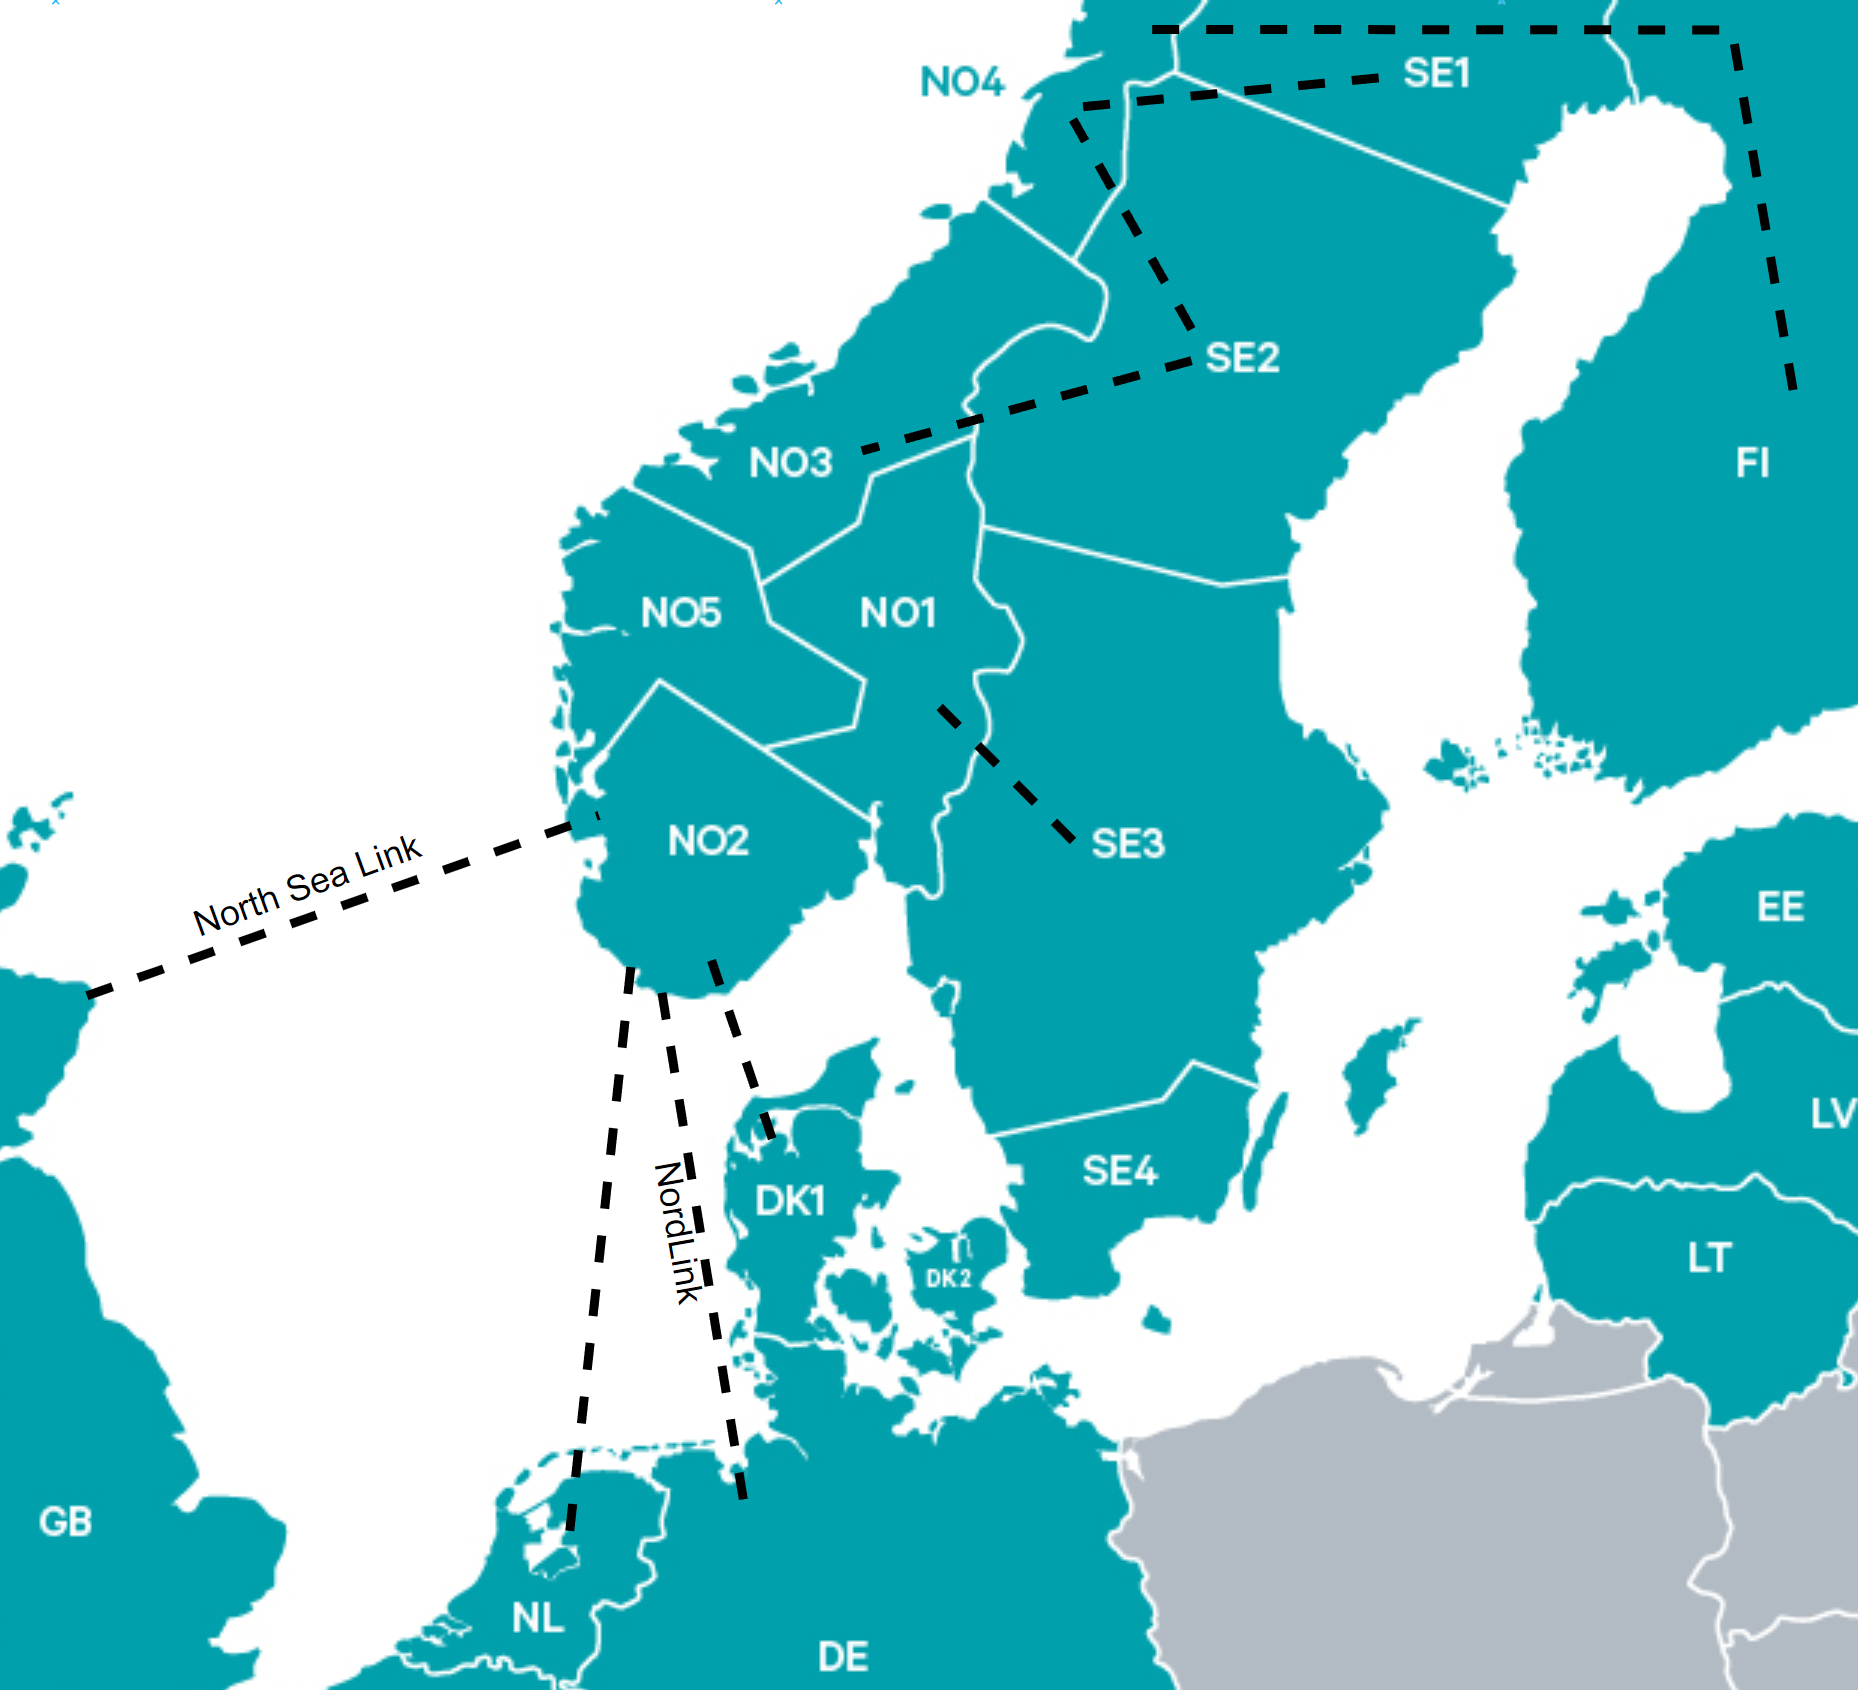
\includegraphics[width=90mm,scale=1.0]{figures/bidding_zones_selfmaid.png}
  \caption{\label{fig:biddin_zones}Bidding zones - https://www.nordpoolgroup.com/the-power-market/Bidding-areas/}

\end{figure}


\begin{figure*}%[t]
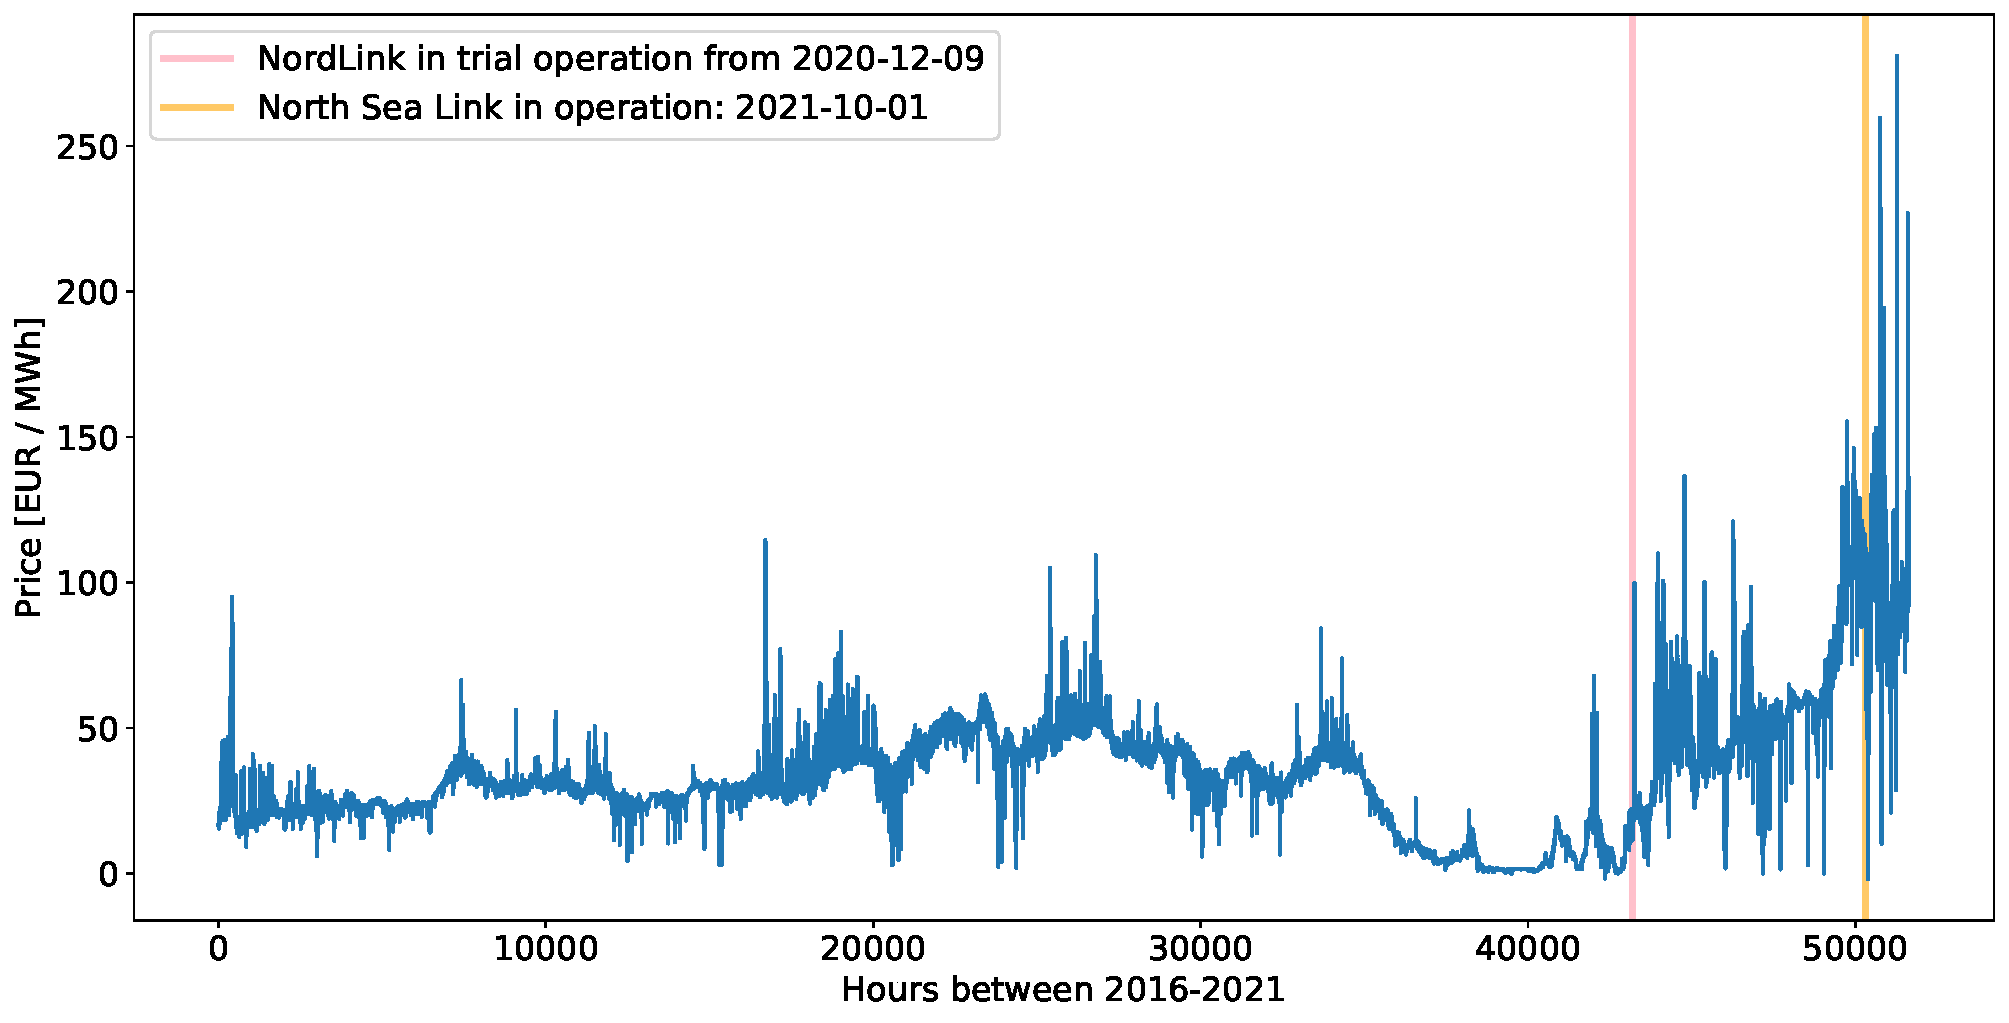
\includegraphics[width=2.0\columnwidth]{figures/price_2016_2021.pdf}
\caption{\label{fig:NO2_price} Electricity price in bidding zone NO2 between 2016 and 2021}
\end{figure*}

In the two previous projects, we studied how spatial and time-independent data could be used to fit an arbitrary function with a given error following the Universal Approximation Theorem \cite{Nielsen2015} using a fully connected Neural Network. However, in Project 3, our data is sequential and time dependant. As such, a fully connected Neural Network is not designed to remember and make use of historical content while feeding forward its current inputs. Therefore, this project will study Recurrent Neural Network and state-of-the-art methods for time-series data.

In the coming sections, we will start off by defining and structuring our dataset, set by the constraints imposed by the different models. Moreover, we briefly cover time-series data and point out the main differences between our data and the Terrain dataset used in Projects 1 and 2. Furthermore, we will develop the framework for both classical statistical models, as well as a sliding window algorithm that can structure our data to be used by both the Feed Forward Neural Network we developed in Project 2 as well as the Recurrent Neural Networks we will study in this Project. After developing our Theory and presenting our Models, we will study their behavior in light of our dataset. Our discussion will cover topics such as central problems regarding RNN performance, such as the unstable gradients and its short term memory as well as comparing the different models with each other. Moreover, we will try to optimize our developed models such that we are able to accurately forecast the electricity price for the next 24 hours. Finally, we will give our final thoughts as we summarize our findings.

\section{Data}
The data used for this project is collected via the Entsoe Transparnecy Platform API. \footnote{https://www.entsoe.eu/data/transparency-platform/}. We also look at "fyllingsgrad" over Norwegian dams, which represents potential power generation. The data is publicaly provided via The Norwegian Energy Regulatory Authority (NVE) \cite{noauthor_magasinstatistikk_nodate}. 
We constructed our own data based on the ones downloaded from the two different APIs. The constucted dataset used for this project can be found in GitHub linked in the appendix, in the data folder. The file used is named MAIN\_DATASET.csv. The file contains 51649 rows and 20 columns containing variables related to power region 2 and 5 in Norway.


\subsection{Market coupling}
\todo[inline]{Bør denne ligge i et annet chp?}
As previously mentioned, the different power markets are being tighter connected thorug interconnecting cables which enables flow of energy between bidding zones and countires. The dotten lines in Figure \ref{fig:biddin_zones} indicates transmission infrastructure, both export and import, 


\subsection{Feature investigation}
Figure \ref{fig:feature_correlation} shows the data and features we focused on and downloaded through the entsoe and NVE API. This include the actual day ahead price, actual and forecasted data of electricity load (demand) and electricity  generation, and the aggrigated "fyllingsgrad" from the dams in zone NO2. "fyllingsgrad" represents electricity that potentially can be produced relative the the amount of water residing within the dam. The delta features were created extra as we wanted to see if forcasted minus actual value would be beneficial. None of the features indicate a significant correlation with respect to the NO2 day ahead price.
\begin{figure}[t]
  \centering
  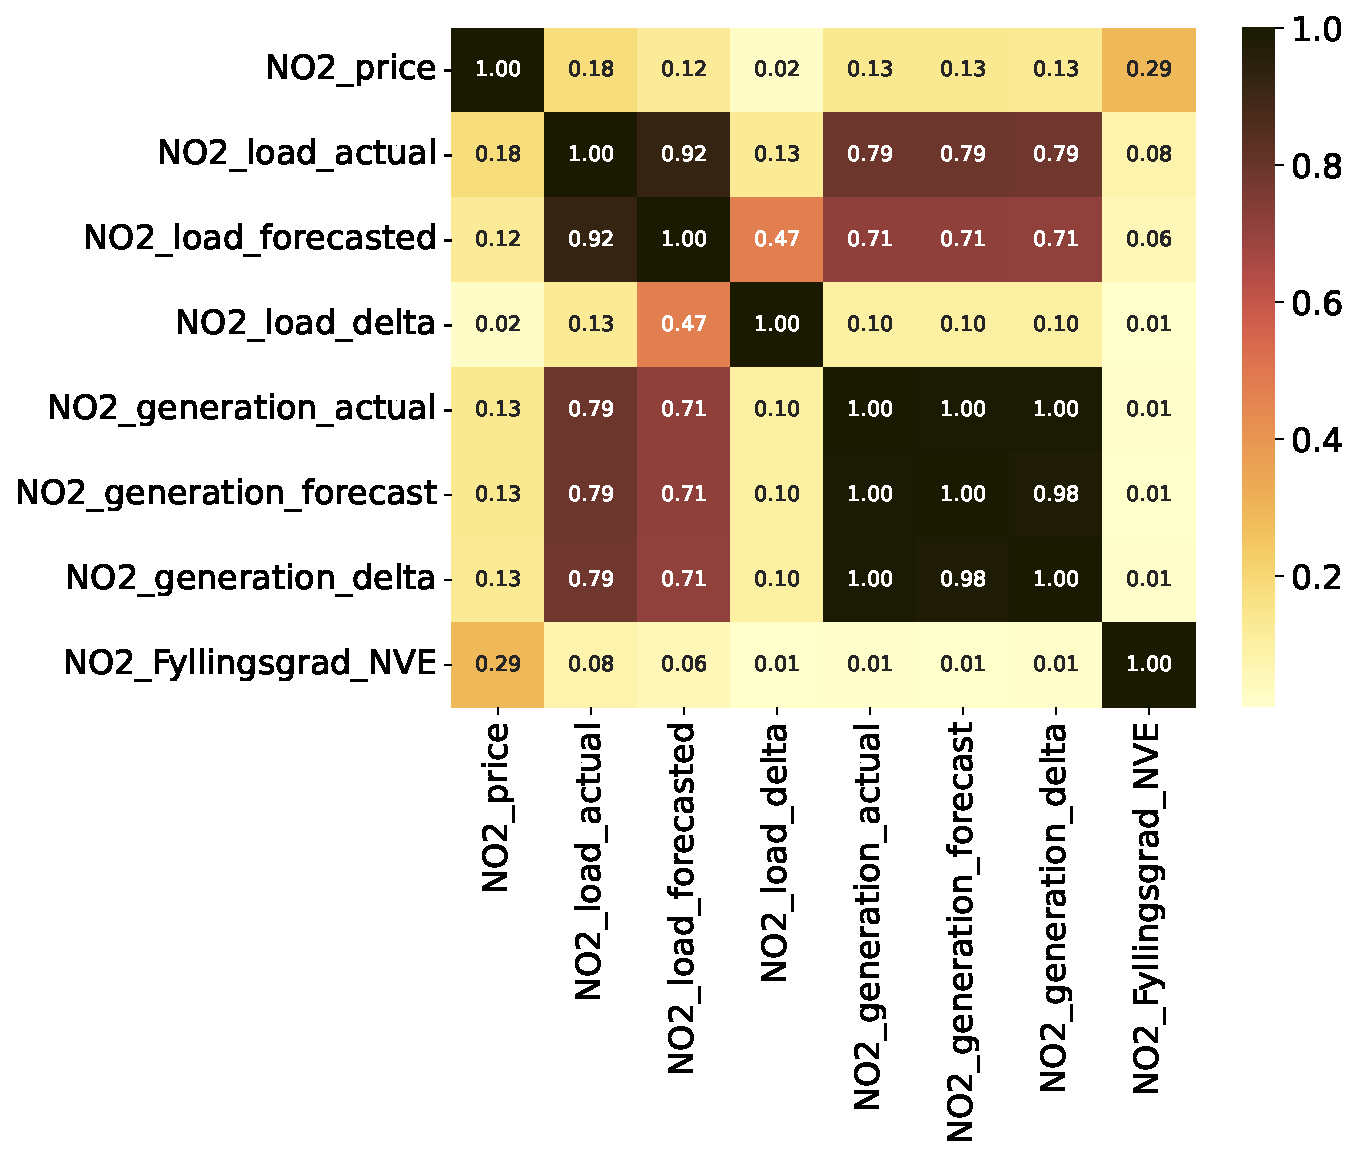
\includegraphics[width=90mm,scale=1.0]{figures/feature_corr_analysis.pdf}
  \caption{\label{fig:feature_correlation}Correlation between data}
\end{figure}

\subsection{Pre-processing}
The dataset has been preprocessed such that it does not contain any NaN values, and the missing values are filled with the previous hours. The data from NVE, "fyllingsrad" initially has weekly time-steps, while the entsoe data has an hourly frequency. Since the nature of the data from NVE, "fyllingsgrad", turned out the be very low-frequency data, we interpolated hourly between weeks to match the hourly time-steps in the entsoe data. Lastly, we shifted the entire dataset to match the closing and opening of the bidding process for the day-ahead market. Thus, our first record starts at 12:00, not 00:00. The electricity price varies within each hour, but the price for the next 24 hours is set at 12:00 the day before. As such, one time-steps for the electricity price is actually 1 day (24 hours) not 1 single hour. It is essential that the model learns the patterns leading up to when Nord pool sets the system price before the market closes and the hourly prices for the next 24 hours are settled. If the model had been trained on intervals between two market days, it would not be synchronized with the power market and our task of forecasts the next day.
\\\\
When feeding data into the RNN, which will be described in greater detail in the coming sections, the data has to be formatted to take the form of the 3D array $\left(\text{Batch Size}, \text{Time Steps}, \text{dimensionality}\right)$. Specifically, Batch Size refers to the number of samples, Time Steps reflect the historical sequence. Finally, dimensionality refers to the number of time series used, such that dimensionality $= 1$ would refer to a univariate time series. Some literature refers to the last dimension as the number of features. We also normalized the data using a minmax scaling, where the data is transformed to fit the range between $0$ and $1$.

\section{Theory and Methods}

\subsection{Data Windowing}
Working with time-series data often requires formulating the time-series data into a supervised learning problem. This can be done by organizing the data into chunks of historical and future data, where the future data is regarded as the target data. This allows for looking back at a sequence of historical data to predict the future. We have applied a sliding window-based algorithm to structure the data into appropriate sample sizes that fit the constraints imposed by converting a time-series data stream to a supervised learning problem fitted for Recurrent Neural Networks. Compared to the previous projects, our data does not contain a relationship between some input data and some target variables; instead, we want to recognize the relationship throughout a sequence of values. Before sectioning the data into windows, we note that our data is evenly spaced which is a requirement for a time-series problem; in our case, we have an hourly time series. Table \ref{tab:sliding_window} visualize an example of how the different chucks of historical and future data can be collected from the original univariate price data stream. $\mathbf{t}$ represents the time step in an hour, $\mathbf{p}$ represents the price at the given time step, and ${n}$ is the last record in the price data stream. The example in table \ref{tab:sliding_window} considers a historical sequence of 4 time-steps indicated by the grey color and a forecast horizon of 2 time-steps indicated as red. Each window including the historical sequence and future data is considered a sample in the constructed windowed dataset. The six leftmoste colums in table \ref{tab:sliding_window} indicates the sliding process with a stride equal to 1. The two right moste columns ilustrates in more detail the lookback and horizon steps including indexing. 

\begin{center}
  \begin{tabular}{|c|c|cc|c|c|cc|c|c|cc|c|c|c}
    \cline{1-2} \cline{5-6} \cline{9-10} \cline{13-14}
    $\mathbf{t}$ & $\mathbf{p}$                  &                &  & $\mathbf{t}$ & $\mathbf{p}$                  &                &  & $\mathbf{t}$ & $\mathbf{p}$                  &                &  & $\mathbf{t}$ & $\mathbf{p}$                      &                \\ \cline{1-2} \cline{5-6} \cline{9-10} \cline{13-14}
    $0$        & \cellcolor[HTML]{C0C0C0}$p_0$ &                &  & $0$        & $p_0$                         &                &  & $0$        & $p_0$                         &                &  & ${0}$   & $p_{0}$                        &                \\ \cline{1-2} \cline{5-6} \cline{9-10} \cline{13-14}
    $1$        & \cellcolor[HTML]{C0C0C0}$p_1$ &                &  & $1$        & \cellcolor[HTML]{C0C0C0}$p_1$ &                &  & $1$        & $p_1$                         &                &  & ${1}$    & $p_{1}$                         &                \\ \cline{1-2} \cline{5-6} \cline{9-10} \cline{13-14}
    $2$        & \cellcolor[HTML]{C0C0C0}$p_2$ &                &  & $2$        & \cellcolor[HTML]{C0C0C0}$p_2$ &                &  & $2$        & \cellcolor[HTML]{C0C0C0}$p_2$ &       &  & $\cdots$    & $\cdots$                         &       \\ \cline{1-2} \cline{5-6} \cline{9-10} \cline{13-14}
    $3$        & \cellcolor[HTML]{C0C0C0}$p_3$ &                &  & $3$        & \cellcolor[HTML]{C0C0C0}$p_3$ &                &  & $3$        & \cellcolor[HTML]{C0C0C0}$p_3$ &       &  & $\cdots$    & $\cdots$                         &       \\ \cline{1-2} \cline{5-6} \cline{9-10} \cline{13-14}
    $4$        & \cellcolor[HTML]{EB7D7D}$p_4$ &                &  & $4$        & \cellcolor[HTML]{C0C0C0}$p_4$ &                &  & $4$        & \cellcolor[HTML]{C0C0C0}$p_4$ &                &  & ${n-4}$    & $p_{n-4}$                         &                \\ \cline{1-2} \cline{5-6} \cline{9-10} \cline{13-14}
    $5$        & \cellcolor[HTML]{EB7D7D}$p_5$ &                &  & $5$        & \cellcolor[HTML]{EB7D7D}$p_5$ &                &  & $5$        & \cellcolor[HTML]{C0C0C0}$p_5$ &       &  & ${n-3}$    & \cellcolor[HTML]{C0C0C0}$p_{n-3}$ &       \\ \cline{1-2} \cline{5-6} \cline{9-10} \cline{13-14}
    $6$        & $p_6$                         &                &  & $6$        & \cellcolor[HTML]{EB7D7D}$p_6$ &                &  & $6$        & \cellcolor[HTML]{EB7D7D}$p_6$ &       &  & ${n-2}$    & \cellcolor[HTML]{C0C0C0}$p_{n-2}$ &       \\ \cline{1-2} \cline{5-6} \cline{9-10} \cline{13-14}
    $7$        & $p_7$                         &                &  & $7$        & $p_7$                         &                &  & $7$        & \cellcolor[HTML]{EB7D7D}$p_7$ &                &  & ${n-1}$    & \cellcolor[HTML]{C0C0C0}$p_{n-1}$ &                \\ \cline{1-2} \cline{5-6} \cline{9-10} \cline{13-14}
    $\cdots$            & $\cdots$                             &                &  & $\cdots$            & $\cdots$                             &                &  & $\cdots$            & $\cdots$                             &                &  & ${n}$    & \cellcolor[HTML]{C0C0C0}$p_{n}$ &       \\ \cline{1-2} \cline{5-6} \cline{9-10} \cline{13-14}
    $\cdots$            & $\cdots$                             &                &  & $\cdots$            & $\cdots$                             &                &  & $\cdots$            & $\cdots$                             &                &  & ${n+1}$    & \cellcolor[HTML]{EB7D7D}$p_{n+1}$ &  \\ \cline{1-2} \cline{5-6} \cline{9-10} \cline{13-14}
    $n$        & $p_n$                         &                &  & $n$        & $p_n$                         &                &  & $n$        & $p_n$                         &                &  & $n+2$        & \cellcolor[HTML]{EB7D7D}$p_{n+2}$     &                \\ \cline{1-2} \cline{5-6} \cline{9-10} \cline{13-14}
  \end{tabular}
  \begin{table}[!h]
    \caption{Visualization of the sliding window process with stide =1, lookback sequence = 4 and horizon = 2}
    \label{tab:sliding_window}
  \end{table}
\end{center}



For our windowed dataset, the window algorithm starts off by sectioning the data into 24-hour chunks, having a stride equal to 24. This allows some flexibility when specifying the input width in terms of a varying number of days. Secondly, a window of length input width and forecast horizon containing 24-hours large cells with a final cell the size of the forecast horizon strides through the chunks with a stride of $1$ day (in other words it moves one chunk at a time). This generates a consecutive sample from our data, which is then restructured together with the other generated consecutive samples to match the required 3D array format imposed by the Recurrent Neural Network.

Since the chunks containing days are repeated in all data windows within the range of the sliding window, we are able to reuse data points in new isolated sequences as the window strides though the chunks. This allows us to effectively increase the number of samples, as contiguous samples contain overlapping data, though differ with regards to the first day used in the input width and data used as forecast horizon. This data window structure allows us to forecast an arbitrarily amount of time ahead, based on the data from a specified number of days ago.

Finally, during train test split, a single data window sample is split in such a way that the input width defines our X (input signal), and the forecast horizon specifies labels y. If the labels y have a length of 1, the RNN is a sequence to vector model predicting a single time step ahead. However, a label vector y with length greater than 1 would not itself specify whether the Recurrent Neural Network is a vector or sequence outputting model, as that would have to be specified in the model declaration. However, a length greater than 1 would indeed indicate that the model is forecasting several time steps ahead. 

\subsection{Time-series and statistical analysis}

\subsubsection{The nature of time series}
As already mentioned, in contrast to projects 1 and 2, this project deals with data in a sequential matter, called time series. What defines this type of format is that the data points decrease, increase or change in chronological order throughout time\cite{Vishwas2020}. A formal definition could be formulated as a mapping from a time-domain to real numbers:

\begin{equation}
  x: T \rightarrow {\rm I\!R}^k 
\end{equation}

where T $\subseteq {\rm I\!R}$ and k $\in \mathbb{N}$ \cite{Auffarth2021}

In the scope of this project, our time series consist of discrete values that describes how several variabels changes over time. These variables are: actual power generation, generation forecast, actual load(demand), load forecast, the delta between forecast and actual and "fyllingsgrad". Dealing with data in such a format might yield additional complexity when trying to analyze the raw data at hand. A widely used yet simple approach for analyzing and forecasting time series includes only the variable destined for forecasting. When analyzing time series on this form, we do not attempt to explain the observed data by the relationship with other possible variables. The only relevant data used for analyzing and forecasting is the past of the variable itself. Data in this format is called a univariate time series, as a contrast to a multivariate time series, which includes several variables connected through a shared period of time. Methods for forecasting the latter will be discussed thoroughly in later sections, but the following section will focus on univariate time series leading up to the Auto-Regressive model, as this works as the most fundamental building block for time series forecasting \cite{Korstanje2021} 

\subsubsection{Decomposing the Characteristics}
As previously mentioned, time series consist of data that describes how different variables change through time. As a result of this aggregation of data, specific characteristics of interest can be decomposed from the original time series. These characteristics can highlight certain aspects of the data in question and help in better the understanding and analysis of the data. To be able to decompose these characteristics, we have made use of the methods implemented in the python module Statsmodels \cite{seabold2010statsmodels}. 


This will help us in visualizing three different components from the time series, in addition to the original data. The first component produced from this method is the trend. This is produced by implementing the method seasonal\_decompose from the Statsmodels module. This method estimates the trend by applying a convolutional filter \cite{seabold2010statsmodels}. 

A trend is a general direction in which something is changing \cite{Auffarth2021}. This trend is, of course, highly dependent on the scope of the time period in question, and the direction of change can differ for different parts of the time series \cite{Vishwas2020}  
Another component that can be highly descriptive for visualizing the time series is the seasonal component. These are patterns in the data with a repeating cyclic variation. After the removal of these components, we are left with the residuals. This is the irregular variation, not explained by the above components\cite{Vishwas2020}.

% decomposed_characteristics
\begin{figure*}
  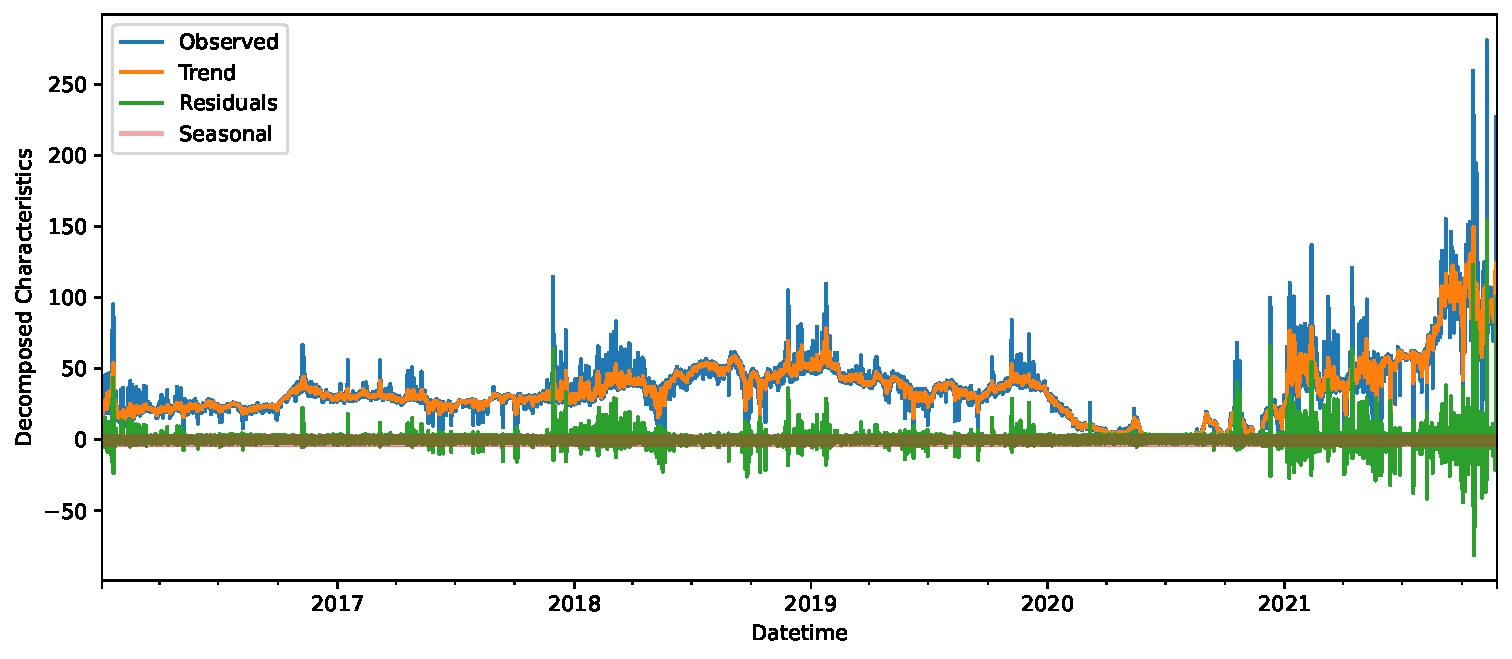
\includegraphics[width=2.1\columnwidth]{figures/decomposed_characteristics.pdf}
  \caption{\label{fig:decomposed_characteristics} Decomposed characteristics of day ahead price NO2}
  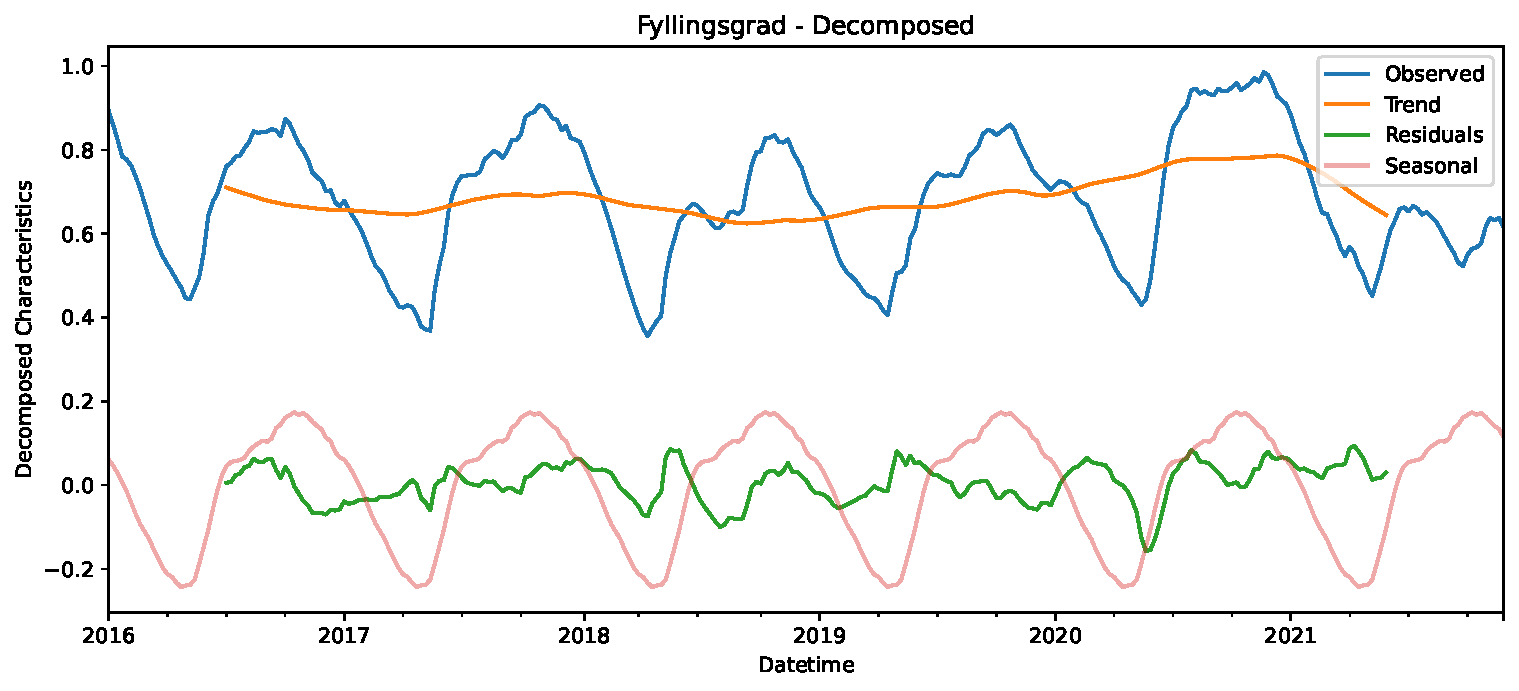
\includegraphics[width=2.1\columnwidth]{figures/NVE_decomposed_characteristics.pdf}
  \caption{\label{fig:NVE_decomposed_characteristics} Decomposed characteristics of NVE "fyllingsgrad"}
\end{figure*}



\subsection{The Auto-Regressive Model}

\subsubsection{Stationarity}
With the different characteristics of the time series decomposed, we move forward with implementing a model with the goal to be able to forecast the price of electricity a given amount of steps ahead in time. As already pointed out, this will be done solely based on the history of the price itself. A general challenge with univariate modeling may arise if the above-mentioned trend is present in the data. If this is the case, the data series is \emph{non-stationary}, and might prove difficult to forecast. As almost every time series will have varying data to some degree, we introduce the Augmented Dickey-Fuller(ADF) test as a statistical test for stationary checking. This is done by implementing the "adfuller" method from Statsmodel \cite{seabold2010statsmodels}. We state a $H_0$ that the unit root is present in the time series.The ADF will return a p-value, where a value smaller than 0.05 will result in the null hypothesis being rejected. Failing to reject this hypothesis will imply that the time series has a non-stationary structure \cite{Vishwas2020}, and will need further processing before being used for forecasting.  

In the case of the latter, a typical method for further preprocessing is the use of differencing. Using this method creates a new time series, consisting of the differences between each value and the following \cite{Korstanje2021}. We can then proceed to compute a new statistical feature, namely autocorrelation. As forecasting with a univariate time series naturally only includes the variable itself, finding patterns on how the past influences the future is crucial. Plotting the autocorrelation gives us a clear visual representation of how the variable is correlated with itself at different time lags. This proves, in other words, a valuable method for determining the linear relationship between time step $t$ and $t-1$ \cite{Vishwas2020}. For the scope of this project, this will give us a measure of how much the price of electricity at a given hour is correlated with the hours ahead. As with regular correlation, the autocorrelation can be both positive and negative \cite{Korstanje2021}. However, the use of \emph{lags} is a concept in autocorrelation that differs from the regular. This notion deals with the number of time steps in which the correlation between each point should be calculated. 
Another vital metric closely connected with autocorrelation is partial autocorrelation. This statistical interpretation of the time series also deals with the correlation between lags, the difference being the latter having removed the effect of in-between time lags\cite{Vishwas2020}. They both are plotted against the specific time lag with a confidence interval, yielding a tool for visually inspecting significant time lags. 

% ACF and PACF
\begin{figure}
  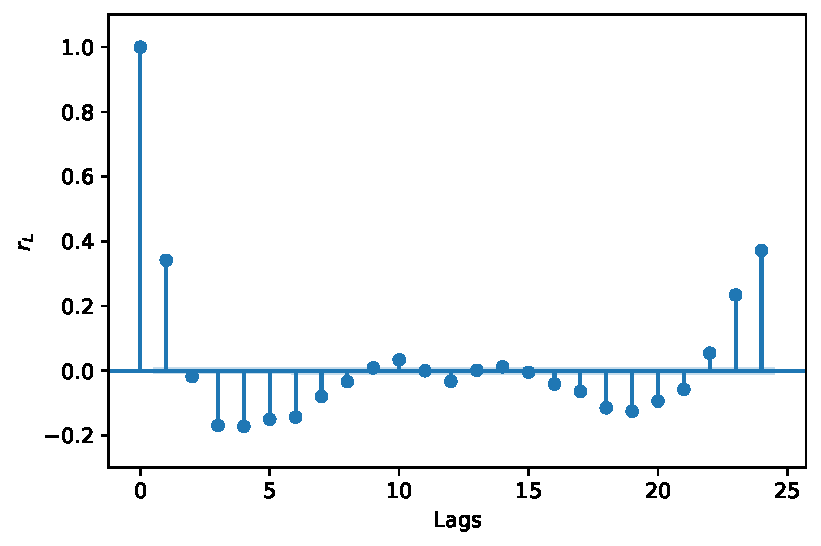
\includegraphics[width=\columnwidth]{figures/AR_acf.pdf}
  \caption{\label{fig:AR_acf} Auto correlation}
  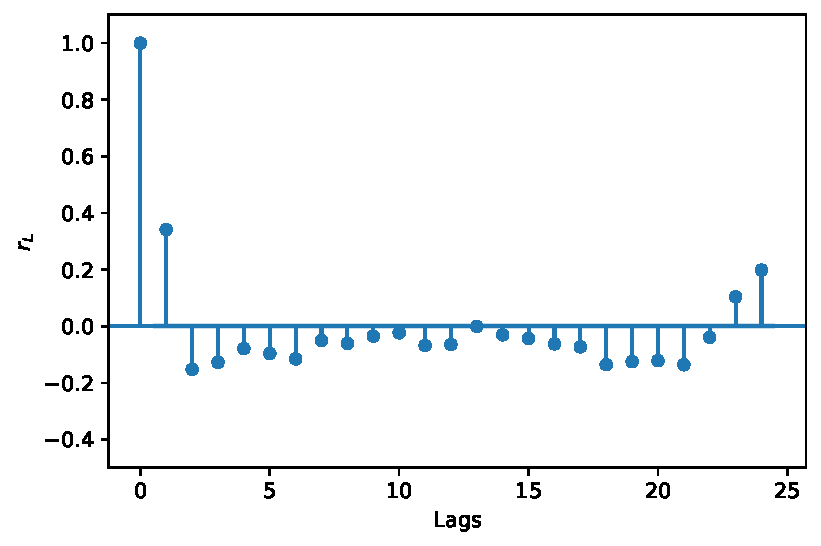
\includegraphics[width=\columnwidth]{figures/AR_pacf.pdf}
  \caption{\label{fig:AR_pacf} Partial auto correlation}
\end{figure}


\subsubsection{Model Definition}

The before mentioned autocorrelation is the basis for the model we then implement for univariate forecasting. At the base of this model is its nature of predicting future variables as a function of the lagged values. This model is formulated as:

\[
X_t = \sum_{i=1}^{p} \phi_i X_{t-i} + \epsilon_{t}
\]

Where $X_t$ is the current time step, $\phi$ is a coefficient for a specific lag, and $\epsilon$ is estimated random noise, for all $p$ time lags \cite{Korstanje2021}. Our implementation of this algorithm can be found in the GitHub repository linked in the Appendix. To estimate the coefficient related to the lag for each time step, we use the Yule-Walker method which consists of the set equations
\begin{equation}
  \label{eq_yw}
  \gamma_m = \sum_{k-1}^p\phi_k\gamma_{m-k} + \sigma_\epsilon^2\delta_{m,0}
\end{equation}
where $\gamma_m$ is the autocovariance function of $X_t$, m is the number of lags from 0 to $p$, $\sigma_\epsilon^2$ is the standard deviation of the Errors and $\delta_{m,0}$ is the Kronecker delta function \cite{Korstanje2021}. Furthermore, we can rewrite this equation as
\begin{equation}
  \nonumber
  \gamma = \Gamma^{-1}\Phi
\end{equation}
where $\gamma \in \mathbb{R}^p$, $\Gamma \in \mathbb{R}^{pxp}$ and $\Phi \in \mathbb{R}^p$. 
which we can solve by applying the Ordinary Least Squares method. By optimizing the equation for $\Phi$ using Ordinary Least Squares, we obtain the expression
\begin{equation}
  \nonumber
  \hat{\Phi} = \left(\Gamma^T\Gamma\right)^{-1}\Gamma^T\gamma
\end{equation}
Where we can use the obtained estimates for our $\phi$'s to find the optimal solution for the $\sigma_\epsilon^2$ in Equation (\ref{eq_yw}), which enables us to fit the AR model.

As previously stated, in this project, our goal is to predict prices for electricity 24 hours ahead. After conducting a grid search, we found that the optimal order of our AR model for solving this problem is 24. This comes as no surprise, as electric pricing has a 24 hours cyclic variation. In this case, where our objective is to forecast multiple time steps, we implemented an iterative approach. As demonstrated by the above equation, the number of previous time steps included in the prediction is dictated by order of the AR model. Our first prediction is, therefore a result of our $\phi$ coefficients being multiplied and summed with actual observed data from the original time series. For a 1 hour prediction, the expected prediction should as a result of this, be fairly accurate. However, when moving further along with the next predicitions, a increasingly larger part of the values from the previous time steps will be predicted values, rather than actual observed. This creates a situation where one runs the risk of aggregating errors throughout the predictions, which is a known weak spot for iterative algorithms of this manner. 

As above equation demonstrates, the AR model of order $p$ needs a total number of $p$ specific $\phi$ coefficients. The optimal value for these coefficients is calculated by fitting the model to the data. To achieve this, we have implemented another function from the Statsmodel module \cite{seabold2010statsmodels}.

\section{Recurrent Neural Networks theory and Methods}

\subsection{Sequence processing using Recurrent Neural Networks}
As our data is sequenced over time, we need a Neural Network that can share its weights across time steps. In a Recurrent Neural Network, this is done by applying the same update rule to the previous output when producing a new output \cite{Goodfellow2016}. Thus, since a Recurrent Neural Network shares its weights across several time steps, it is suitable to use for temporal data then a standard FeedForward Neural Network as touched upon in the introduction.

Mathematically, we can define this system as
\begin{equation}
  \nonumber
  \bm{s}^{(t)} = f(\bm{s}^{(t-1)},\bm{x}^{(t)};\bm{\theta})
\end{equation}
Where $\bm{s}^{(t)}$ is the state of the system, $\bm{x}^{(t)}$ is an external signal which drives the system and $\bm{\theta}$ parametrizes $f$, though we note that this system itself does not contain any output. 

Recurrent Neural Networks support multiple different input and output sequences \cite{Geron2019}. A tuple of inputs or outputs over different time steps is considered a sequence, whereas a input or output from a singular time step is considered a vector. RNNs support different constellations of sequence/vector input and output, such that it is possible to input a sequence and output a sequence where some time steps are ignored. This is a favorable property given our data and task of producing a full day forecast some time steps after the end of our input sequence.

\subsection{Backpropagation through time}
Though computing the gradient through a Recurrent Neural Network is analogous to how it was computed in a Feed Forward Neural Network, the algorithm has to be applied throughout all the time steps of the Recurrent Neural Network recursively. The recursion starts at the final time step, where at the final time step $\tau$ the gradient of the loss $L$ can be computed as follows, using the notation of \cite{Goodfellow2016}
\begin{equation}
  \nabla_{\bm{h}^{(\tau)}}L = \bm{V}^T \nabla_{\bm{o}^{(\tau)}}L
\end{equation}
where $\bm{V}$ is the weights between the hidden states and output values $\bm{o}$.
Going backwards trough time ($t < \tau)$, the gradient of the propagated loss can be computed using the following equation
\begin{equation}
  \bm{W}^TJ(\bm{a})(\nabla_{\bm{h}^{(t+1)}}L)+\bm{V}^T(\nabla_{\bm{o}^{(t)}}L)
\end{equation}
where $\bm{W}$ is the weights associated with the hidden-to-hidden state connection and $J(\bm{a})$ is the jacobian of the activation function.%


Given a long time sequence, a Recurrent Neural Network can be both memory and cpu intensive. Moreover, for long sequences of data, the unrolled RNN will be a considerably deep Neural Network. As we discussed in Project 2, a deep Neural Network is prone to the unstable gradient problem, where the gradient can either completely vanish or explode through the bounds of the datatype used to contain the value. In addition to the RNN being prone to unstable gradients given a long sequence, the memory of the first inputs will deter if the RNN is processing a long sequence \cite{Geron2019}.

\subsection{The unstable gradient problem}
Our main motivation behind introducing different activation functions such as the ReLU and Leaky ReLU to replace the Sigmoid activation function in Project 2 was to avoid the vanishing gradient which arose from the bounded output from the Sigmoid. However, a non-saturated activation function such as the ReLU family of functions runs the risk of updating the set of weights between two layers in such a way that the computed output is slightly increased. For a Feed Forward Neural Network, given how additional sets of weights are computed during gradient descent, this weight update pattern is not given to reoccur. Though for a Recurrent Neural Network, the same sets of weights are updated at every time step, such that a weight update pattern that ends up in a slight increase of the output would be reapplied until the output explodes \cite{Geron2019}. As such, when implementing a Recurrent Neural Network in the coming Section, we will use a saturating activation function such as the Hyperbolic Tangent $\tanh = \frac{\sinh}{\cosh}$, which conveniently is supplied as the default activation function for RNNs in TensorFlow \cite{tensorflow2015-whitepaper}.

\subsection{The Short-Term memory problem}
The second problem which arises in the context of training a Recurrent Neural Network is its inevitable memory loss of the earliest states as a result of how some information is lost for each time step \cite{Geron2019}. By following the approach of \cite{Hochreiter1997}, implementing Long Short-Term Memory (LSTM) cells can alleviate the memory loss. The idea behind LSTM cells is to store some information in the long-term, while at the same time forget unnecessary information whilst reading the rest which result in the short term output memory. In this way, for each time step some information is kept, while at the same time some long term memories are dropped if they meet certain requirements after each time step \cite{Geron2019}. As such, LSTM cell can be able to recognize, preserve, utilize and abolish trends in the data as needed, acheiving a better mean squared error than for the simple RNN cell. 
Another gated RNN which might alleviate the short term memory problem of Recurrent Neural Networks is the Gated Recurrent Unit, which simplifies the LSTM cell by combining the forget and output gate into one single gate \cite{Goodfellow2016}. additionally, the GRU cell merges both the long term memory state and the hidden state into a single vector. Though a GRU cell would outperform an LSTM cell in terms of computational efficiency \cite{Geron2019}, GRU as well as other gated RNNs derived from the LSTM cell performs approximately the same as LSTM \cite{Greff2015}.
A long sequence can also be shortened by applying a 1-dimensional convolutional layer as a pre-processing layer, before passing the shortened signal on to an RNN. Given our current application, the convolutional layer will effectively downsample a given input sequence, given the size of the convolutional kernel \cite{Geron2019}. The convolutional layer will both detect structures in the sequence as well as shortening the sequence. This in turn can benefit the RNN in terms of its memory, as it will be able to remember longer sequences than in the absence of a preprocessing convolutional layer.
Another preprocessing layer which might improve the performance of a RNN is a FeedForward layer. The FeedForward layer will project the input into a feature space with temporal dynamics, which may yield improved performance. \cite{Murugan2018}

Throughout this project, we will study both the effect of the aforementioned architectural differences, namely the difference between a sequence to vector and sequence to sequence RNN when predicting several time steps ahead. Furthermore, we will also study the effect of the different preprocessing techniques outlined above in response to both the gradient and memory loss problem. All in context of the ENTSOE dataset. 

\subsection{Setting up our RNN}
What follows is the basic structure that our developed RNN models will attain, following the constraints and conditions outlined in the previous sections. For clarity, all RNNs will be developed using the Keras frontend of TensorFlow \cite{tensorflow2015-whitepaper}. For a complete implementation of the models, we refer to the GitHub linked in the Appendix. 

We have developed models that are able to forecast a single, as well as several time steps ahead in time both via a vector and sequence approach. The main difference between a sequence to vector and sequence to sequence in terms of the RNN architecture is how the final recurrent layer returns its output. For a sequence to vector model, the only the final output node is considered, whereas for a sequence to sequence model we set the \textit{return\_sequences} flag to \textbf{True} as that would return all computed output nodes distributed through time. Finally, regardless of model architecture, a regular Dense feed forward layer distributes the output of the Recurrent Layer according to the specified forecast Horizon. Note that a Dense layer in TensorFlow supports sequences as input, meaning that it can handle the output from a recurrent layer regardless of vector or sequence form \cite{Geron2019}. 

A preprocessing layers such as a 1-dimensional convolution layer or a FeedForward layer can be implemented akin to the layers discussed above, taking the place as the input layer for their specific model.

As stated previously, the hyperbolic tangent function is sufficient as activation function for an RNN due to its saturating property. As such, our RNNs will default to the hyperbolic tangent as activation function. Moreover, an adaptive learning rate optimizer during gradient descent is chosen. For our models, we will default to the ADAM optimizer.

\section{Results}
We note that all results have been created with the Source Code found in the Appendix. The results are reproducible, for further explanation for how to run the code and reproduce the results, refer to the README in the GitHub. All color maps used have been developed to fairly represent all data, with an emphasis of being readable for those with visual deficiency \cite{Crameri2021}. 

\subsection{Auto Regressive Model}
% grid search AR
\begin{figure}
  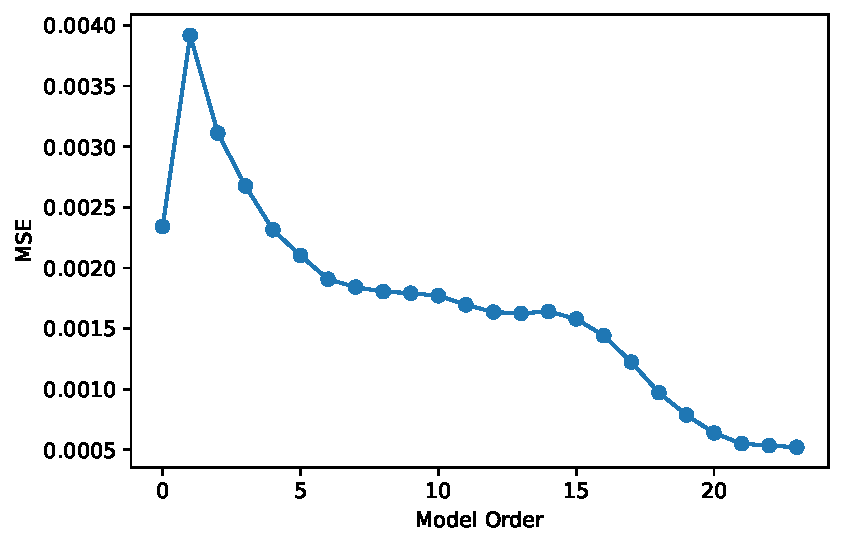
\includegraphics[width=\columnwidth]{figures/AR_gridsearch.pdf} 
  \caption{\label{fig:AR_gridsearch} AR grid search on order $p$}
\end{figure}

% AR-model on order 24
\begin{figure*}
  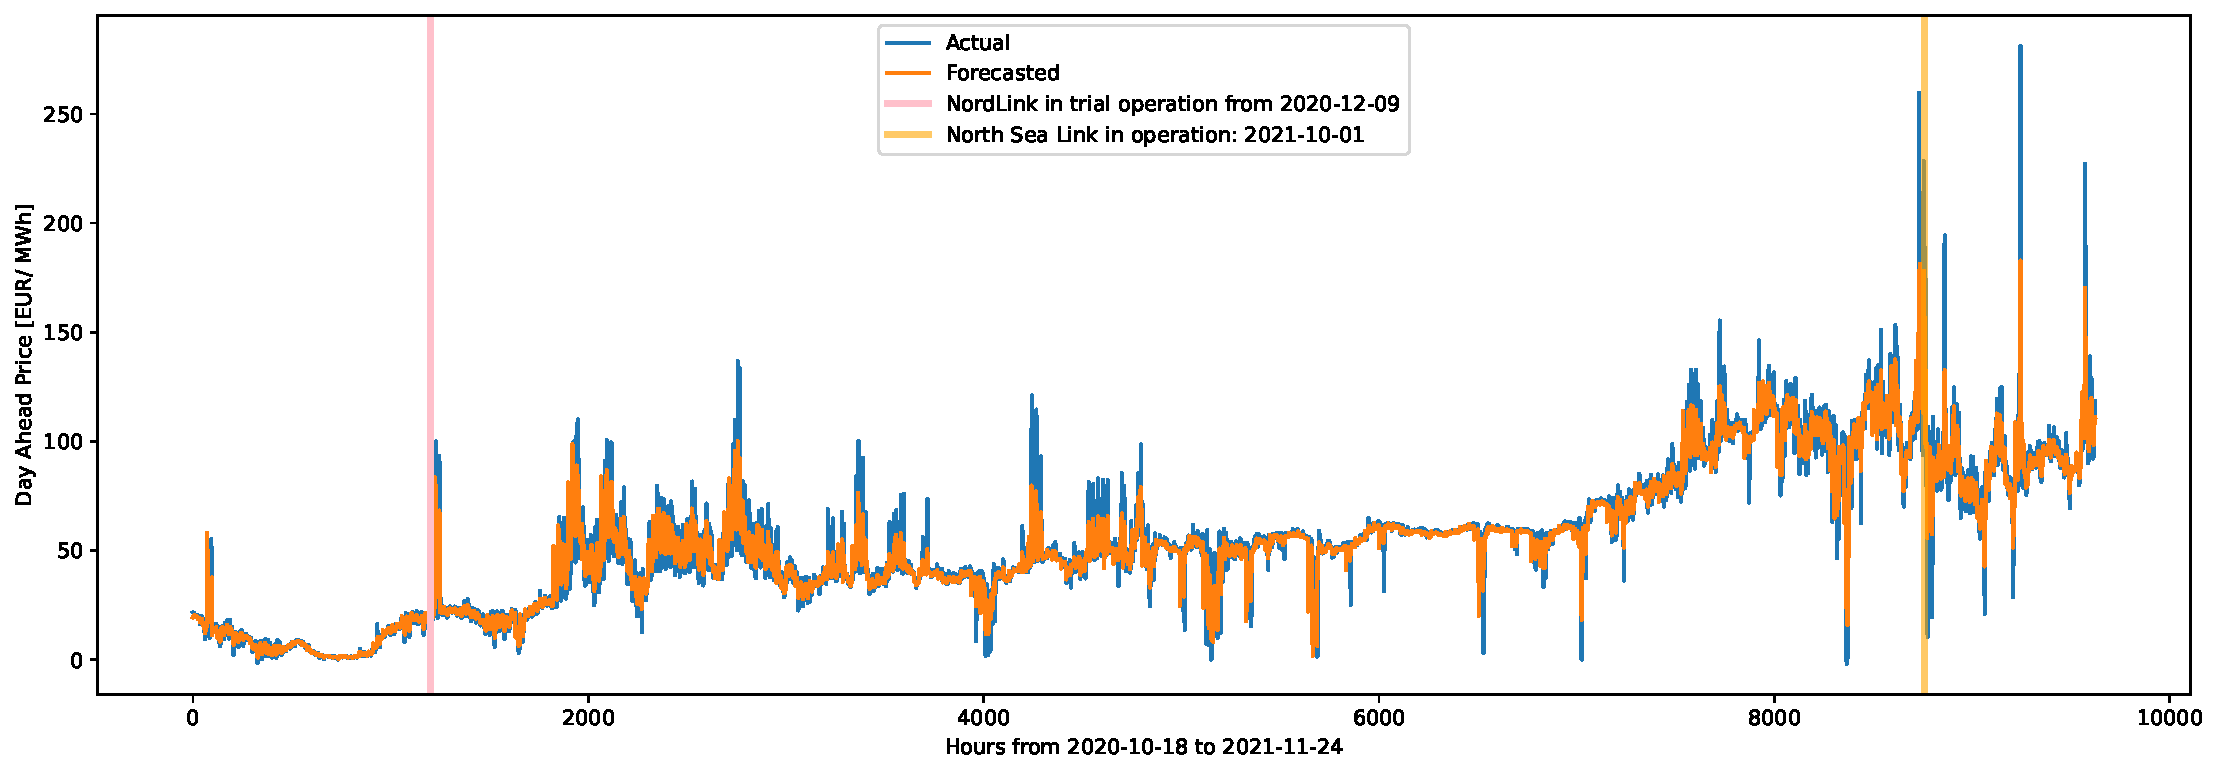
\includegraphics[width= 2.1\columnwidth]{figures/AR(24)_daily predictions.pdf} 
  \caption{\label{fig:AR(24)_daily predictions} AR-model(24), 24 hour forecast)}
  
\end{figure*}





\subsection{Recurrent Neural Networks}

\subsubsection{Behaviour of uni -and multivariate models}
These results are part of a preliminary study to determine how the different Recurrent Neural Network Cells respond to a change in number of neurons. For all results, each model is created equal according to the choice of parameters, except for the Cell structure. In the univariate case, only price is used. Moreover, in the multivariate case, forecasted values and actual values are assigned to specific models. For clarity, no results show the inclusion of the NVE \"fyllingsgrad\" data. All results for the current subsection are made using a Sequence to Sequence model.

% Training evaluation
\begin{figure}
  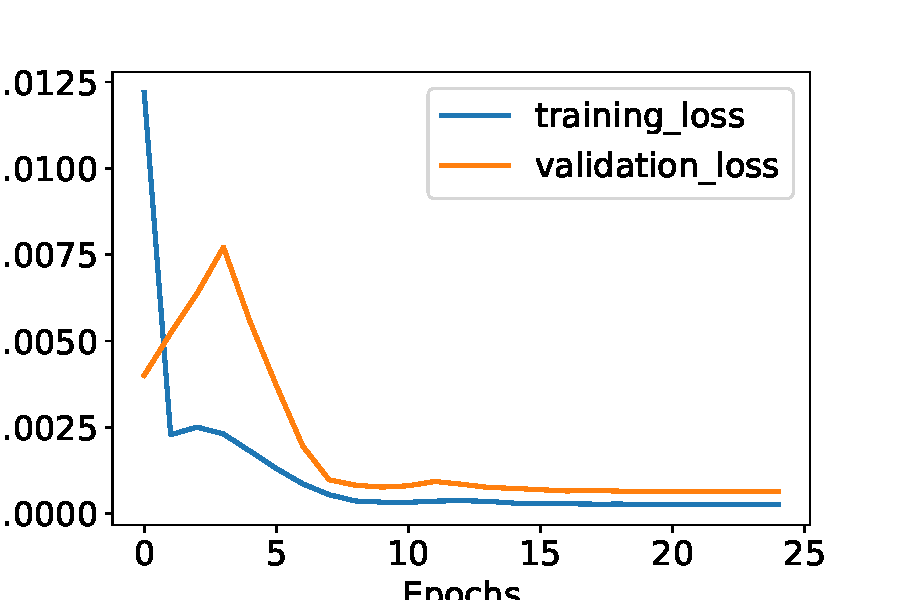
\includegraphics[width=\columnwidth]{figures/univariate_train_evaluation_RNN.pdf}
  \caption{\label{fig:univariate_train_evaluation_RNN} Univariate train evaluation RNN}
  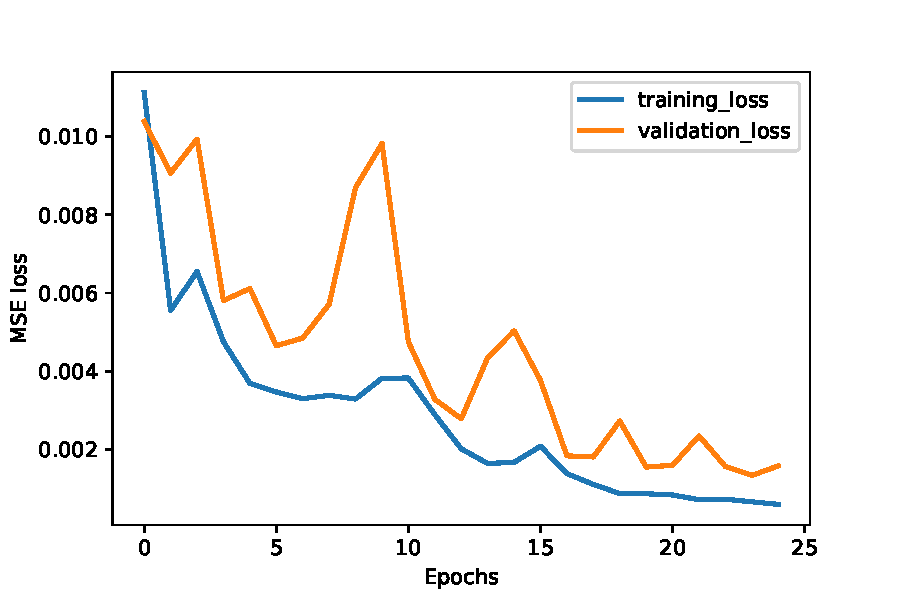
\includegraphics[width=\columnwidth]{figures/univariate_train_evaluation_convGRU.pdf}
  \caption{\label{fig:univariate_train_evaluation_ConvGRU} Univariate train evaluation conv GRU}
  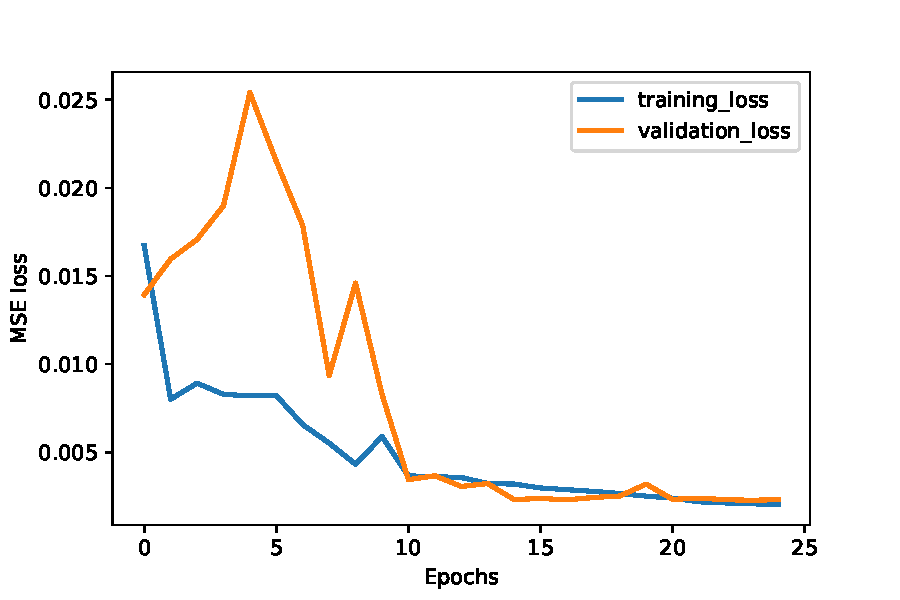
\includegraphics[width=\columnwidth]{figures/univariate_train_evaluation_LSTM.pdf}
  \caption{\label{fig:univariate_train_evaluation_LSTM} Univariate train evaluation LSTM}
\end{figure}

\begin{figure}
  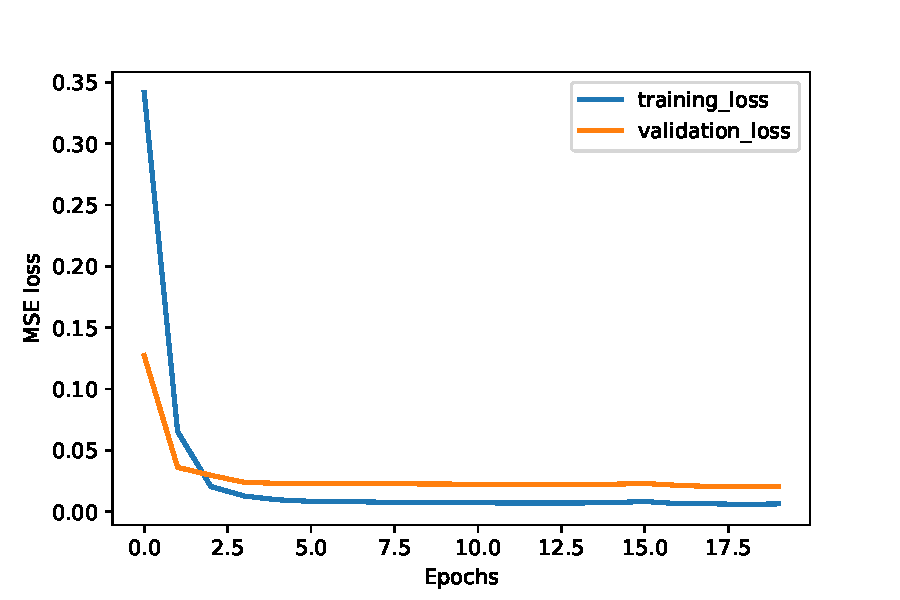
\includegraphics[width=\columnwidth]{figures/multivariate_train_evaluation_RNN.pdf}
  \caption{\label{fig:multivariate_train_evaluation_RNN} multivariate train evaluation RNN}
  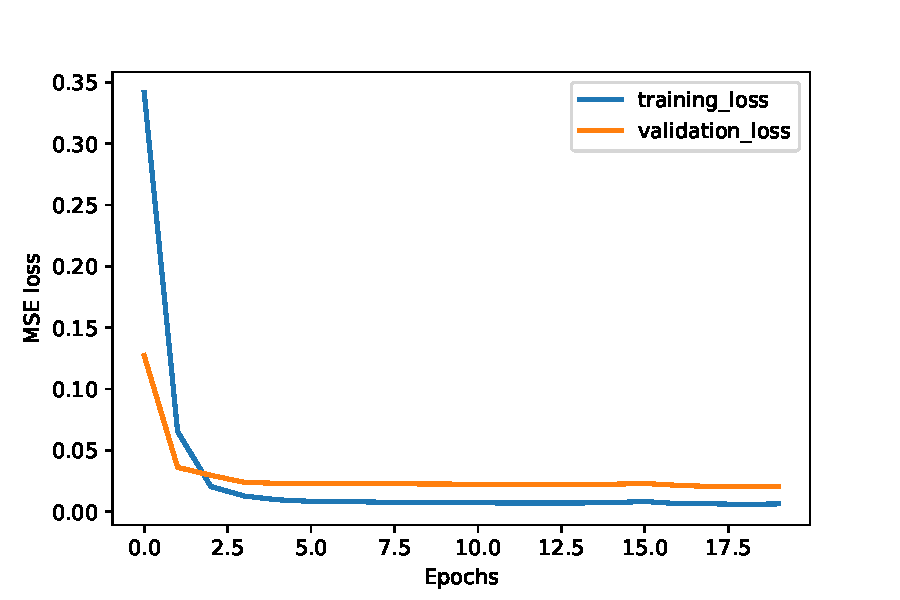
\includegraphics[width=\columnwidth]{figures/multivariate_train_evaluation_RNN.pdf}
  \caption{\label{fig:multivariate_train_evaluation_ConvGRU} multivariate train evaluation conv GRU}
  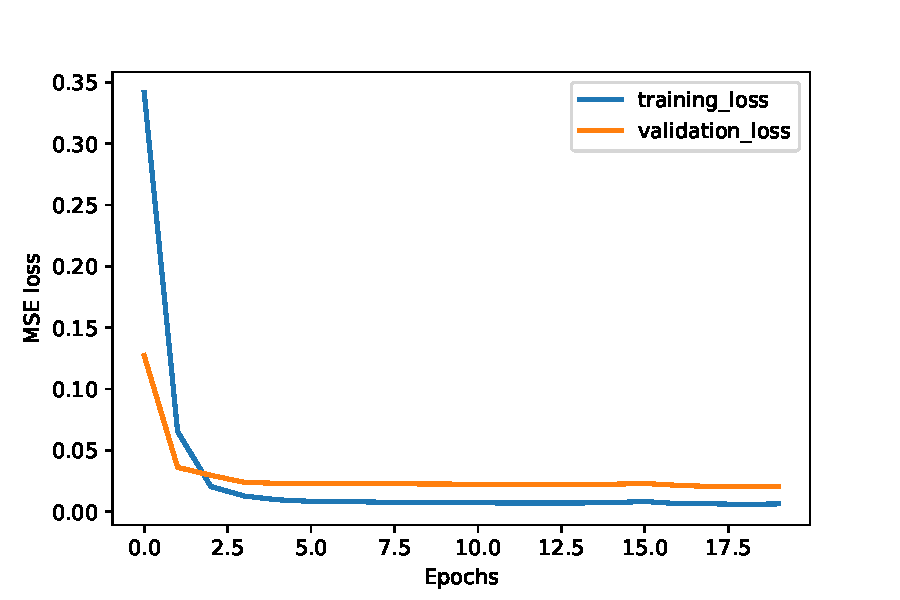
\includegraphics[width=\columnwidth]{figures/multivariate_train_evaluation_RNN.pdf}
  \caption{\label{fig:multivariate_train_evaluation_LSTM} multivariate train evaluation LSTM}
\end{figure}

% Hourly statistics
\begin{figure}
  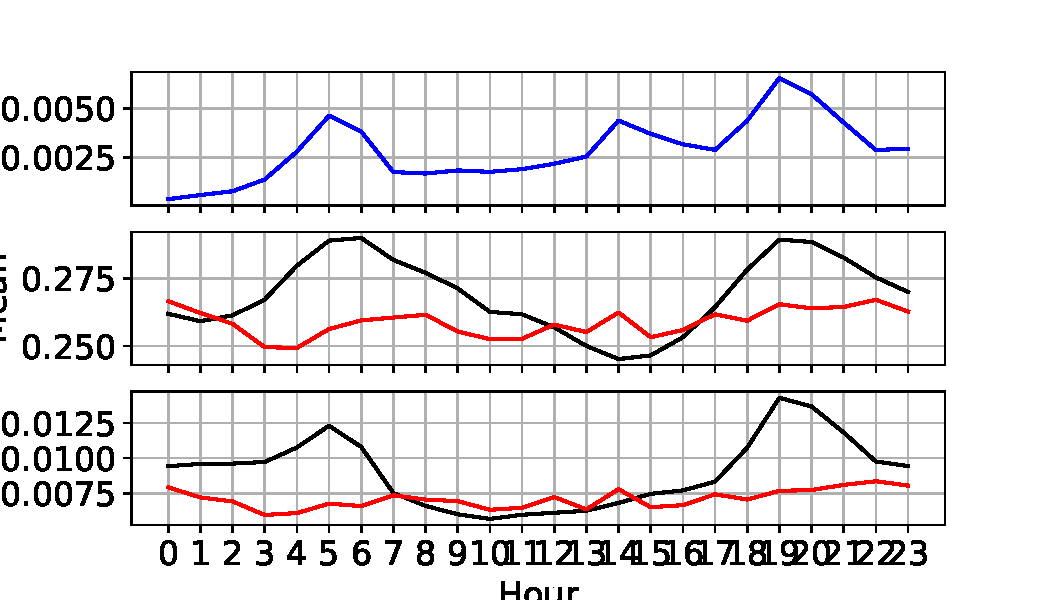
\includegraphics[width=\columnwidth]{figures/univariate_hourly_stats_RNN.pdf}
  \caption{\label{fig:univariate_hourly_stats_RNN} Univariate Simple RNN performance - Blue color indicate MSE for spesific hours. Black indicate mean and variance of target, and red indicate mean and variance of all predictions relative to its hour}
  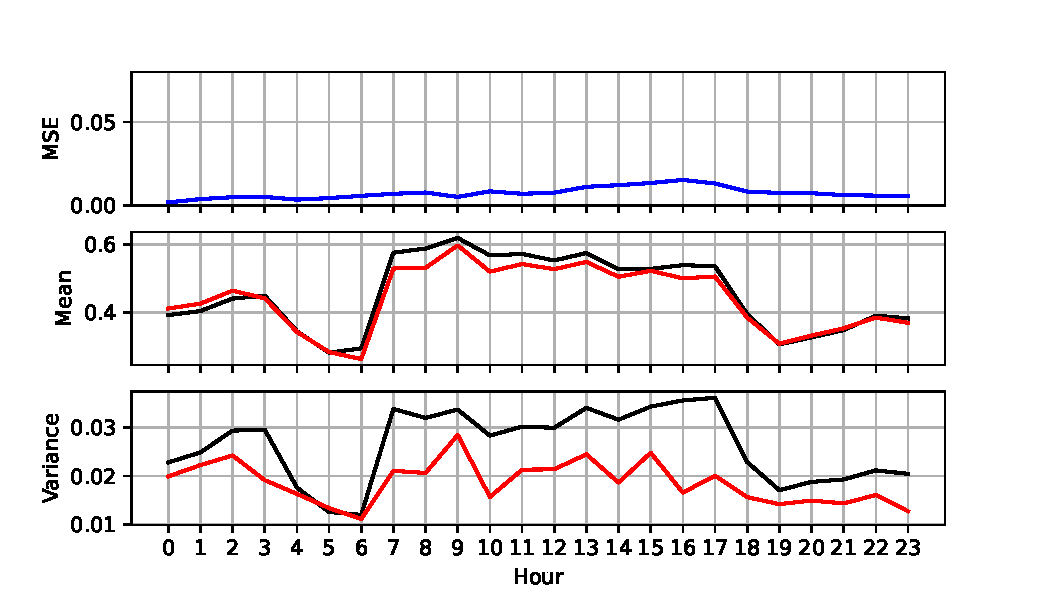
\includegraphics[width=\columnwidth]{figures/univariate_hourly_stats_convGRU.pdf}
  \caption{\label{fig:univariate_hourly_stats_convGRU} Univariate ConvGRU performance - Blue color indicate MSE for spesific hours. Black indicate mean and variance of target, and red indicate mean and variance of all predictions relative to its hour}
  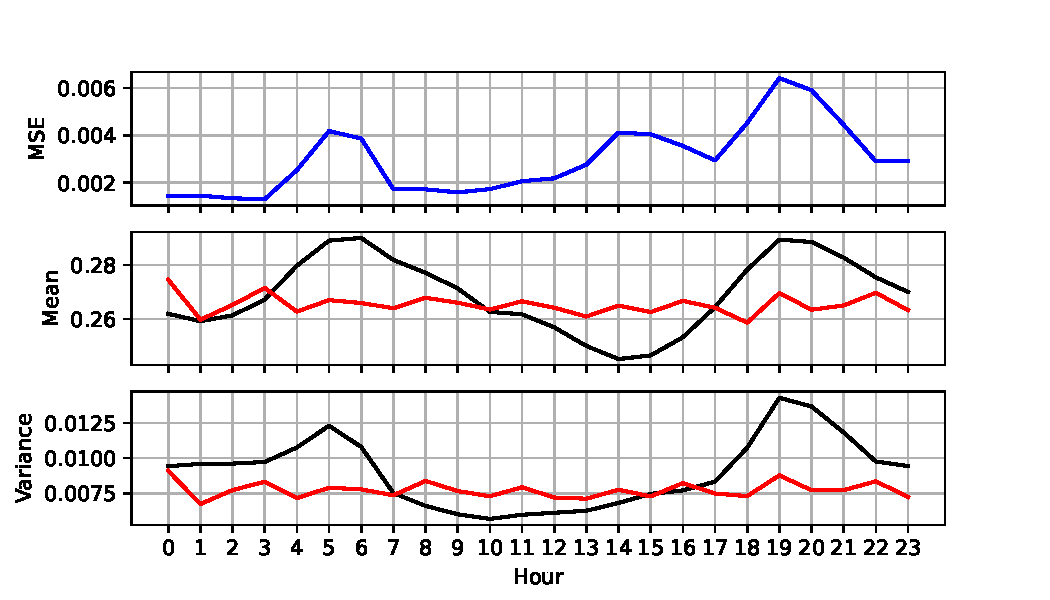
\includegraphics[width=\columnwidth]{figures/univariate_hourly_stats_LSTM.pdf}
  \caption{\label{fig:univariate_hourly_stats_LSTM} Univariate LSTM performance - Blue color indicate MSE for spesific hours. Black indicate mean and variance of target, and red indicate mean and variance of all predictions relative to its hour}
\end{figure}

\begin{figure}
  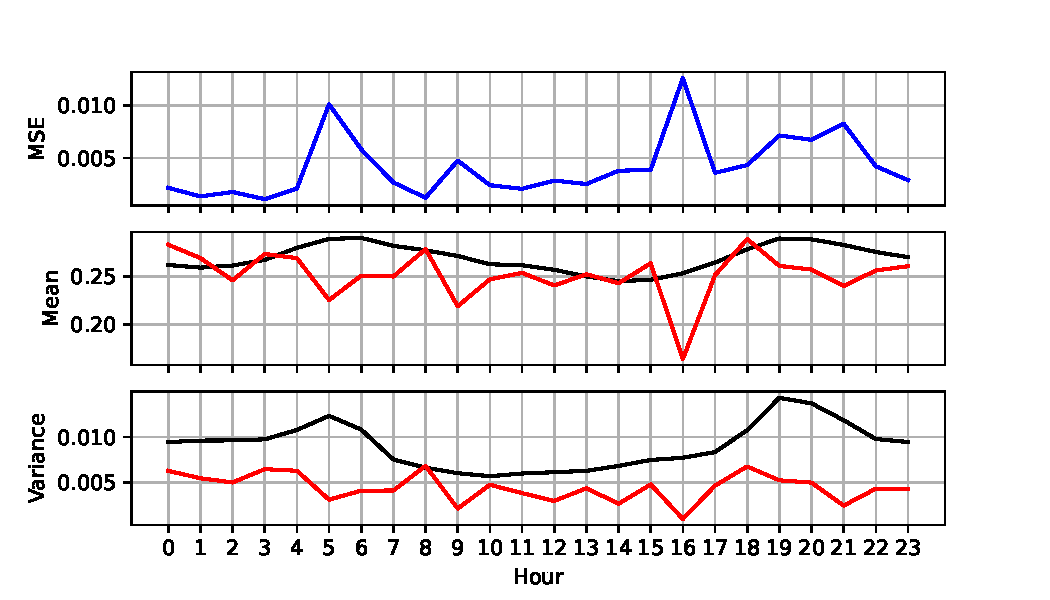
\includegraphics[width=\columnwidth]{figures/multivariate_hourly_stats_RNN.pdf}
  \caption{\label{fig:multivariate_hourly_stats_RNN} Multivariate Simple RNN performance - Blue color indicate MSE for spesific hours. Black indicate mean and variance of target, and red indicate mean and variance of all predictions relative to its hour}
  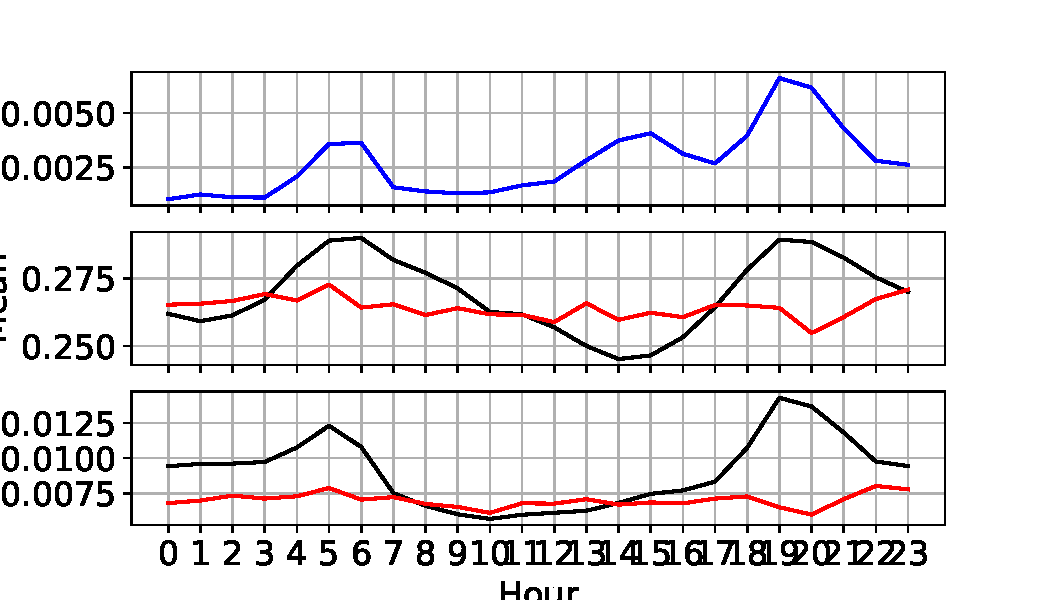
\includegraphics[width=\columnwidth]{figures/multivariate_hourly_stats_convGRU.pdf}
  \caption{\label{fig:multivariate_hourly_stats_convGRU} Multivariate ConvGRU performance - Blue color indicate MSE for spesific hours. Black indicate mean and variance of target, and red indicate mean and variance of all predictions relative to its hour}
  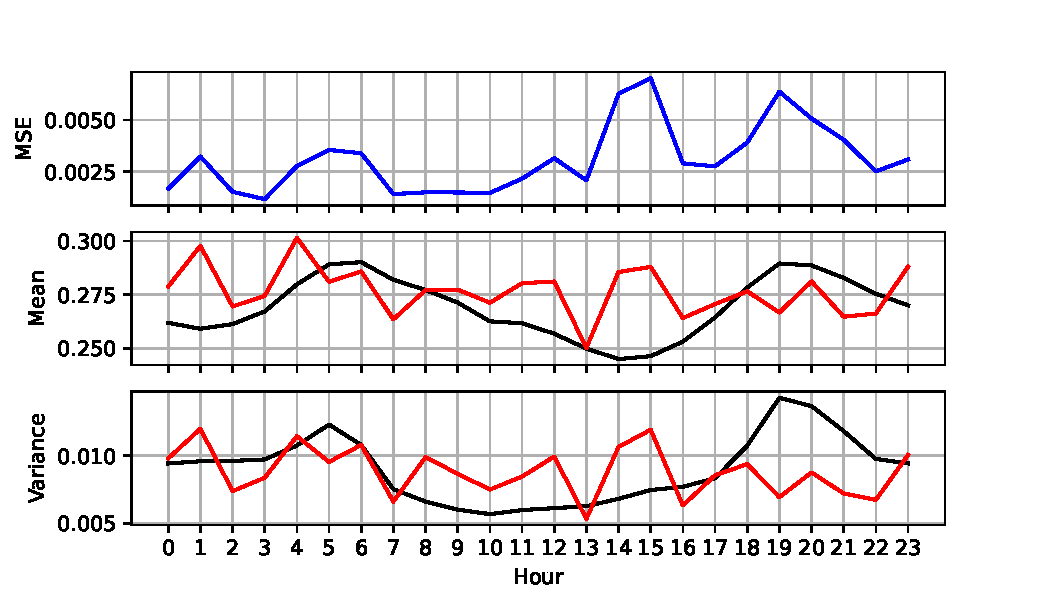
\includegraphics[width=\columnwidth]{figures/multivariate_hourly_stats_LSTM.pdf}
  \caption{\label{fig:multivariate_hourly_stats_LSTM} Multivariate LSTM performance - Blue color indicate MSE for spesific hours. Black indicate mean and variance of target, and red indicate mean and variance of all predictions relative to its hour}
\end{figure}


% Best univariate predictions
\begin{figure}
  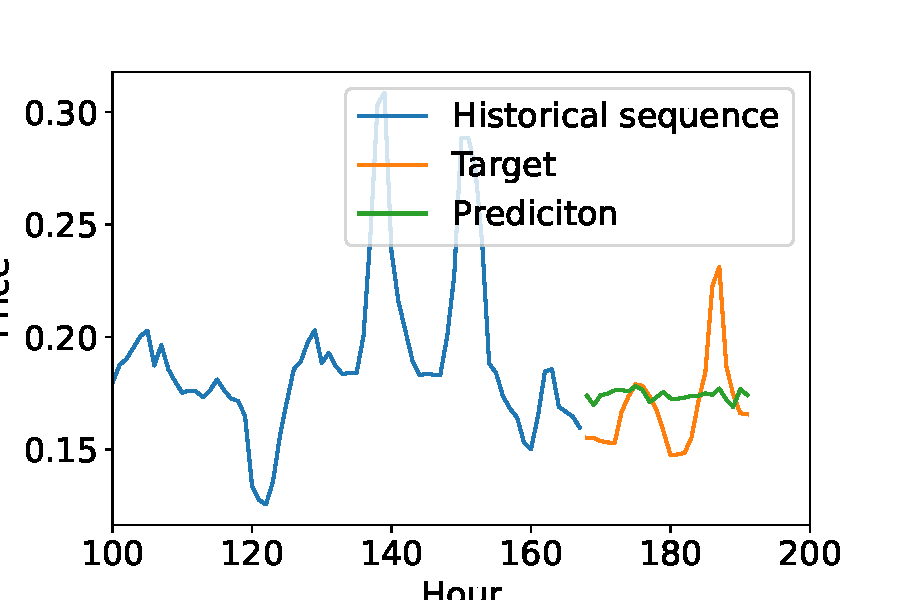
\includegraphics[width=\columnwidth]{figures/univariate_predictions_convGRU_testsample11.pdf}
  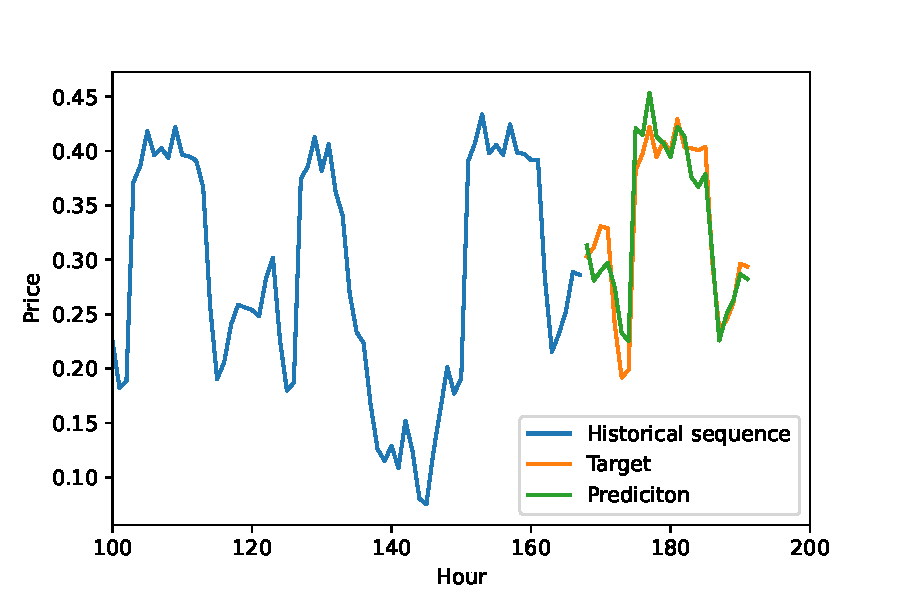
\includegraphics[width=\columnwidth]{figures/univariate_predictions_convGRU_testsample24.pdf}
  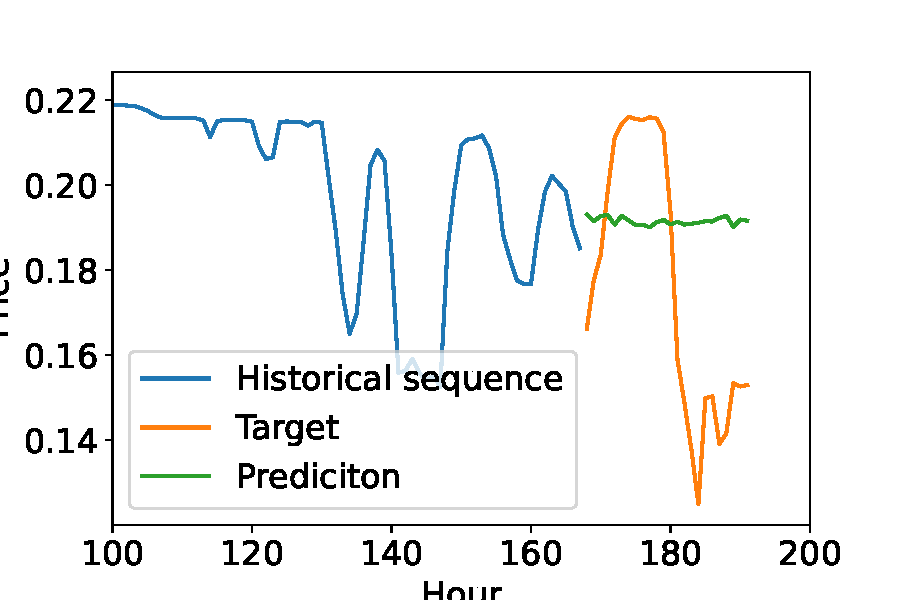
\includegraphics[width=\columnwidth]{figures/univariate_predictions_convGRU_testsample98.pdf}  
  \caption{\label{fig:univariate_best_predictions} Three sample predictions from the best univariate model GRU with 1d convolution}
\end{figure}

% Best multivariate predictions
\begin{figure}
  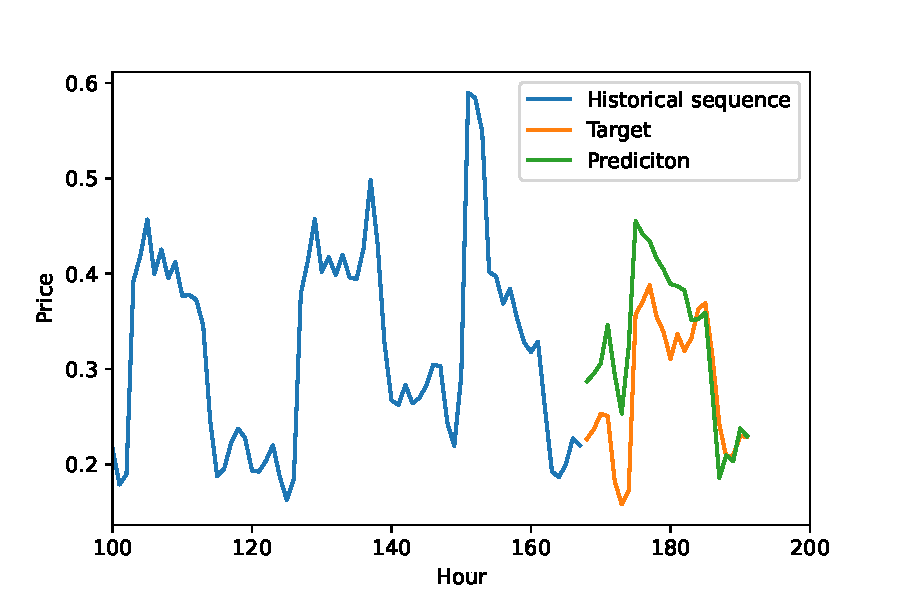
\includegraphics[width=\columnwidth]{figures/multivariate_predictions_convGRU_testsample11.pdf}
  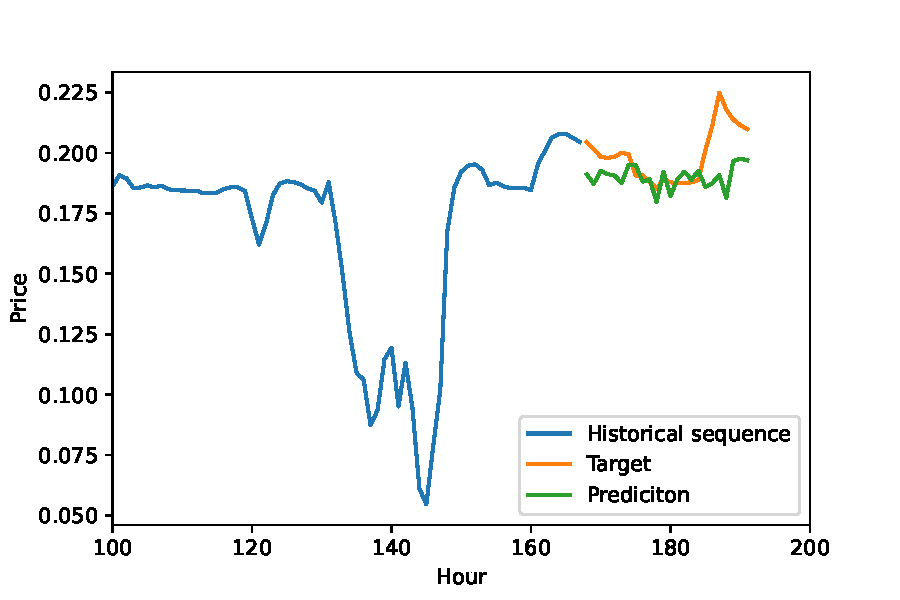
\includegraphics[width=\columnwidth]{figures/multivariate_predictions_convGRU_testsample24.pdf}
  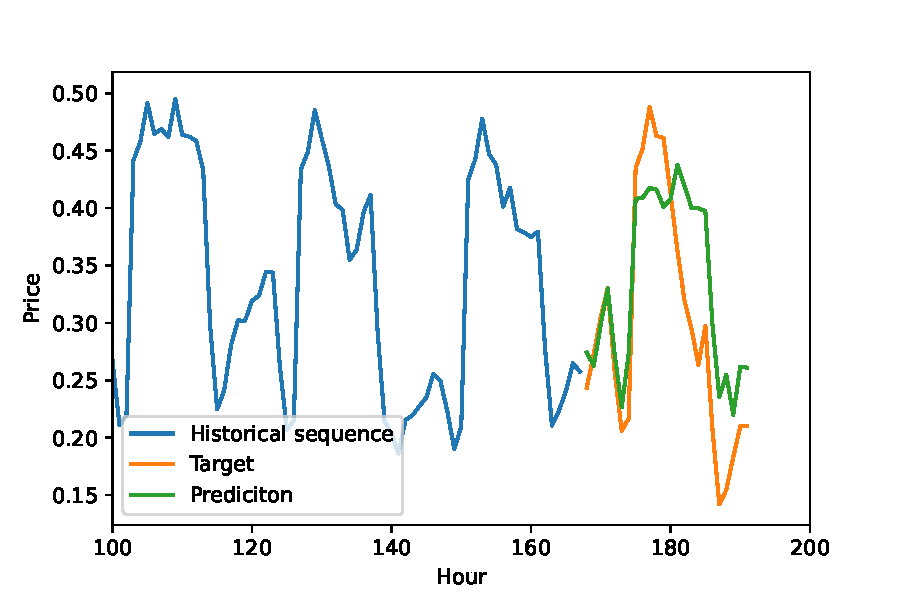
\includegraphics[width=\columnwidth]{figures/multivariate_predictions_convGRU_testsample98.pdf}  
  \caption{\label{fig:multivariate_best_predictions} Three sample predictions from the best multivariate model GRU with 1d convolution}
\end{figure}


\begin{figure}
  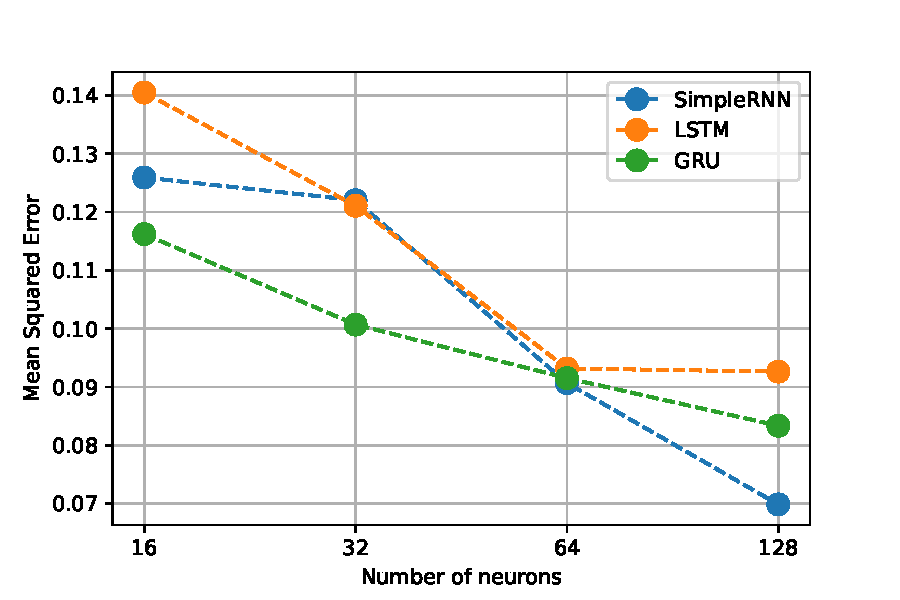
\includegraphics[width=\columnwidth]{figures/small_architecture_grid_search.pdf}
  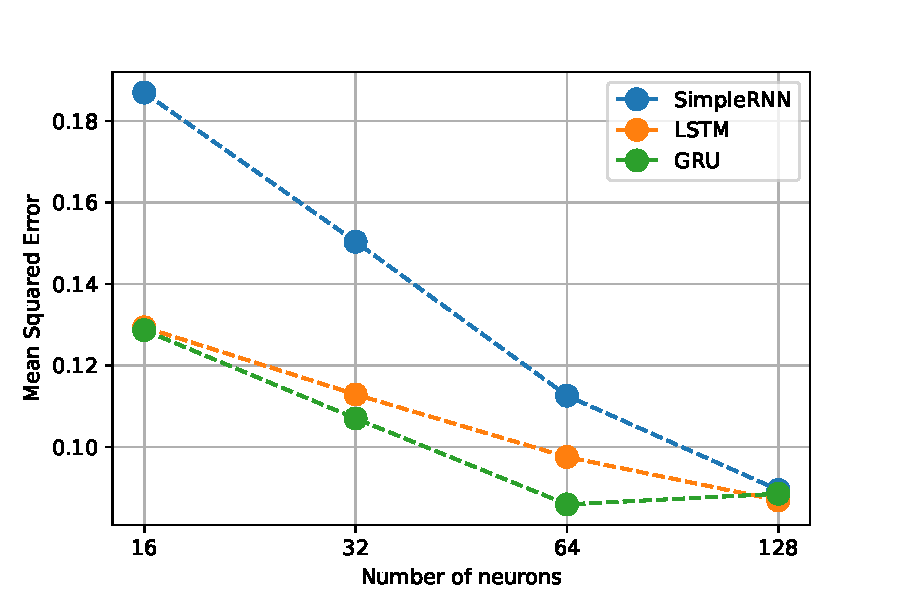
\includegraphics[width=\columnwidth]{figures/multivariate_forecast_small_architecture_grid_search.pdf}
  \caption{\label{fig_smallgs}Mean Squared Error as function of number of neurons for a single layer model. The uppermost figure shows a univariate case, while the plot at the bottom shows for a multivariate case}
\end{figure}

Figure (\ref{fig_smallgs}) shows the Mean Squared Error as a function of number of Neurons for a single layered, univariate model. Whereas Figure (\ref{fig_smallmultigs}) shows the Mean Squared error for the same models, but this time using a multivariate input of price, forecast load and forecast generation.

\begin{figure}
  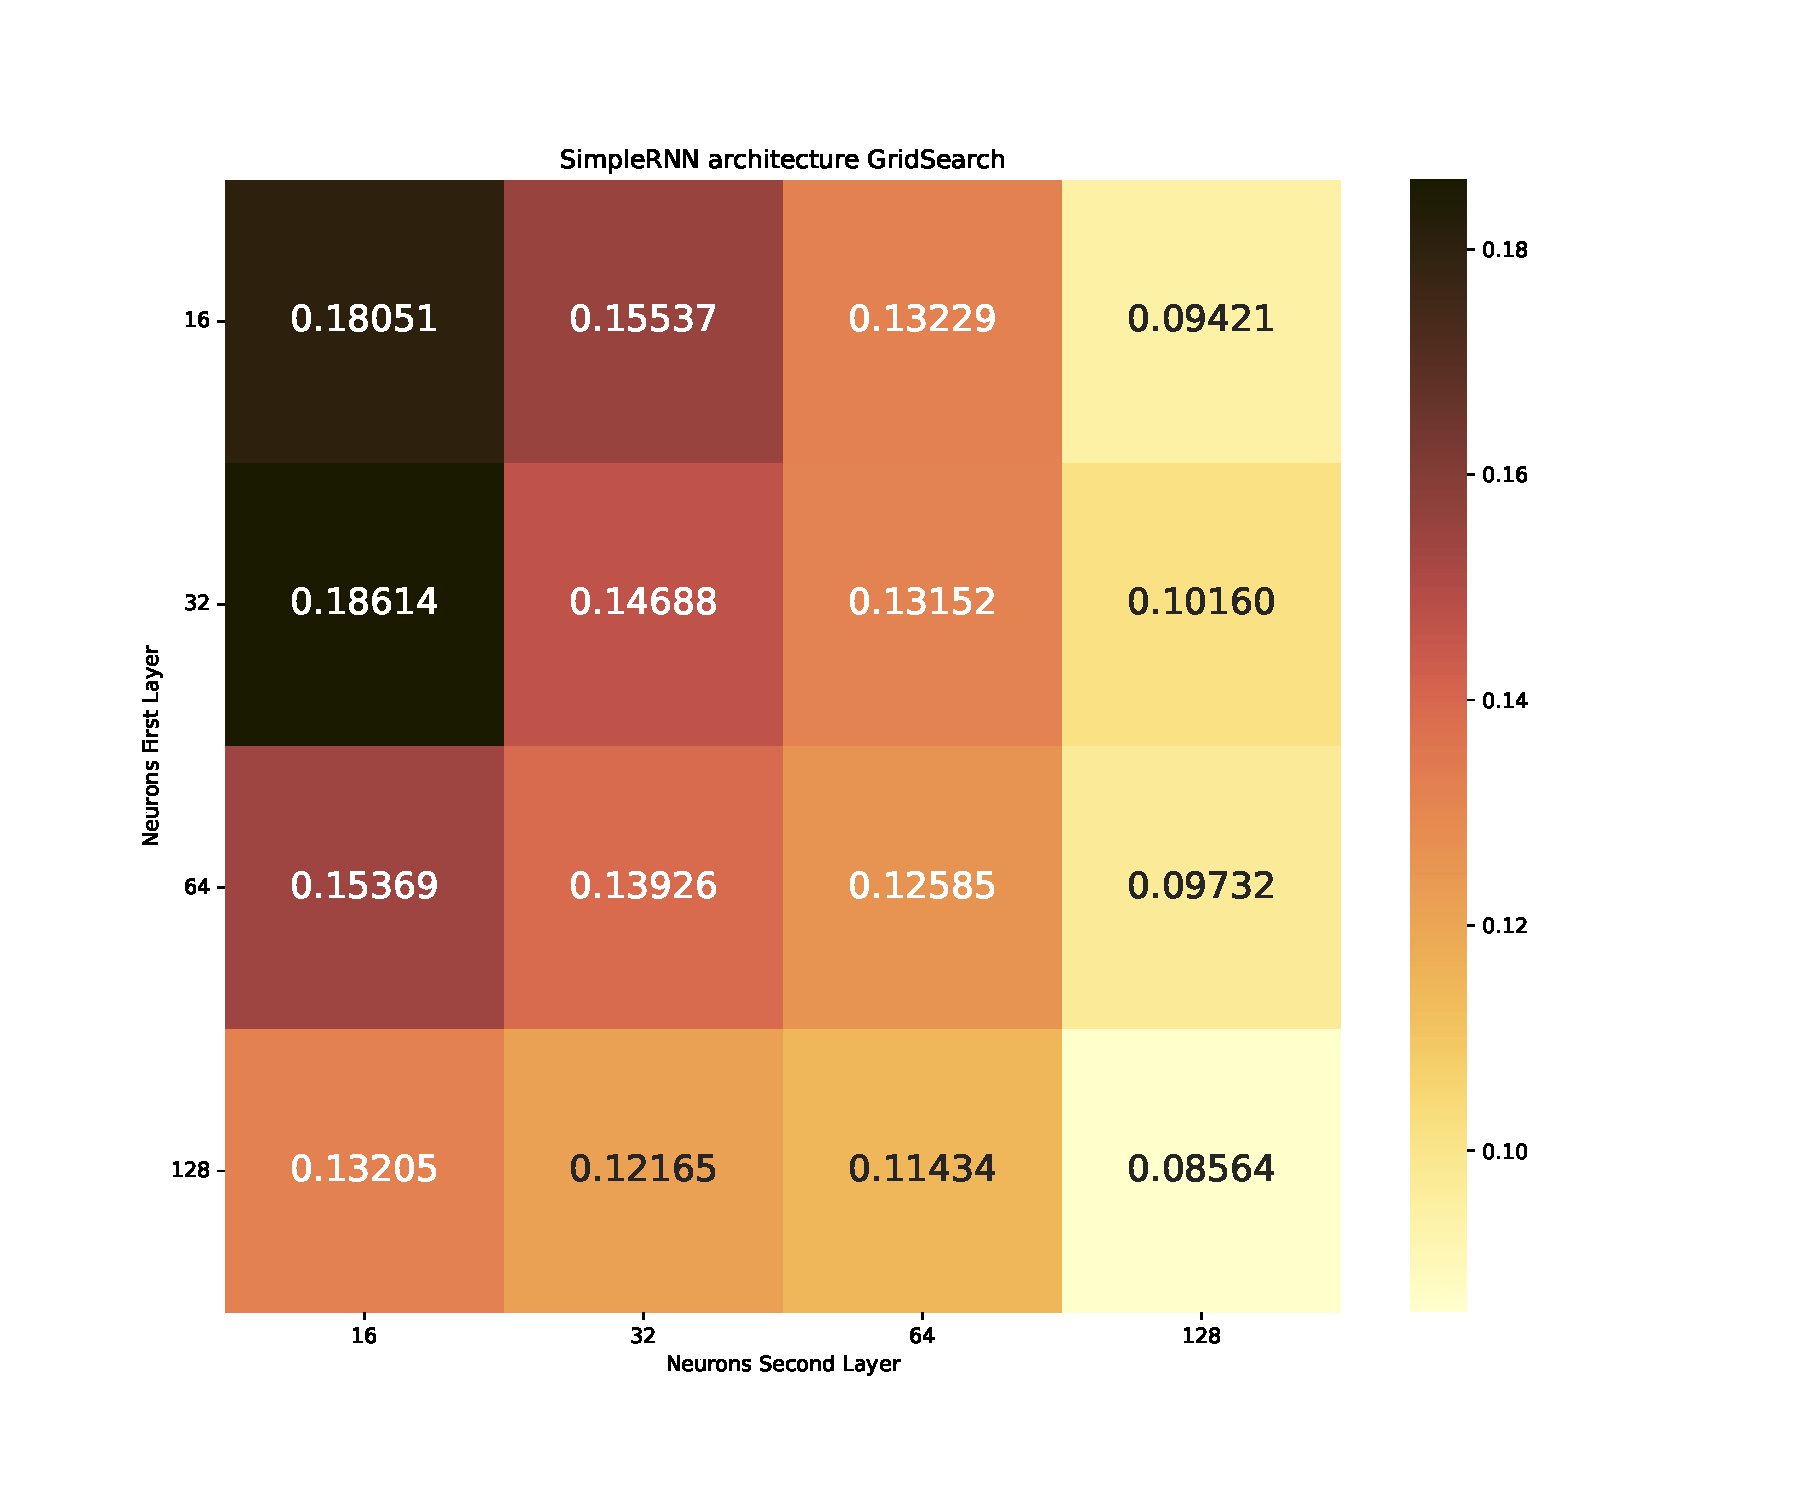
\includegraphics[width=\columnwidth]{figures/Large_forecast_gridsearch_rnn.pdf}
  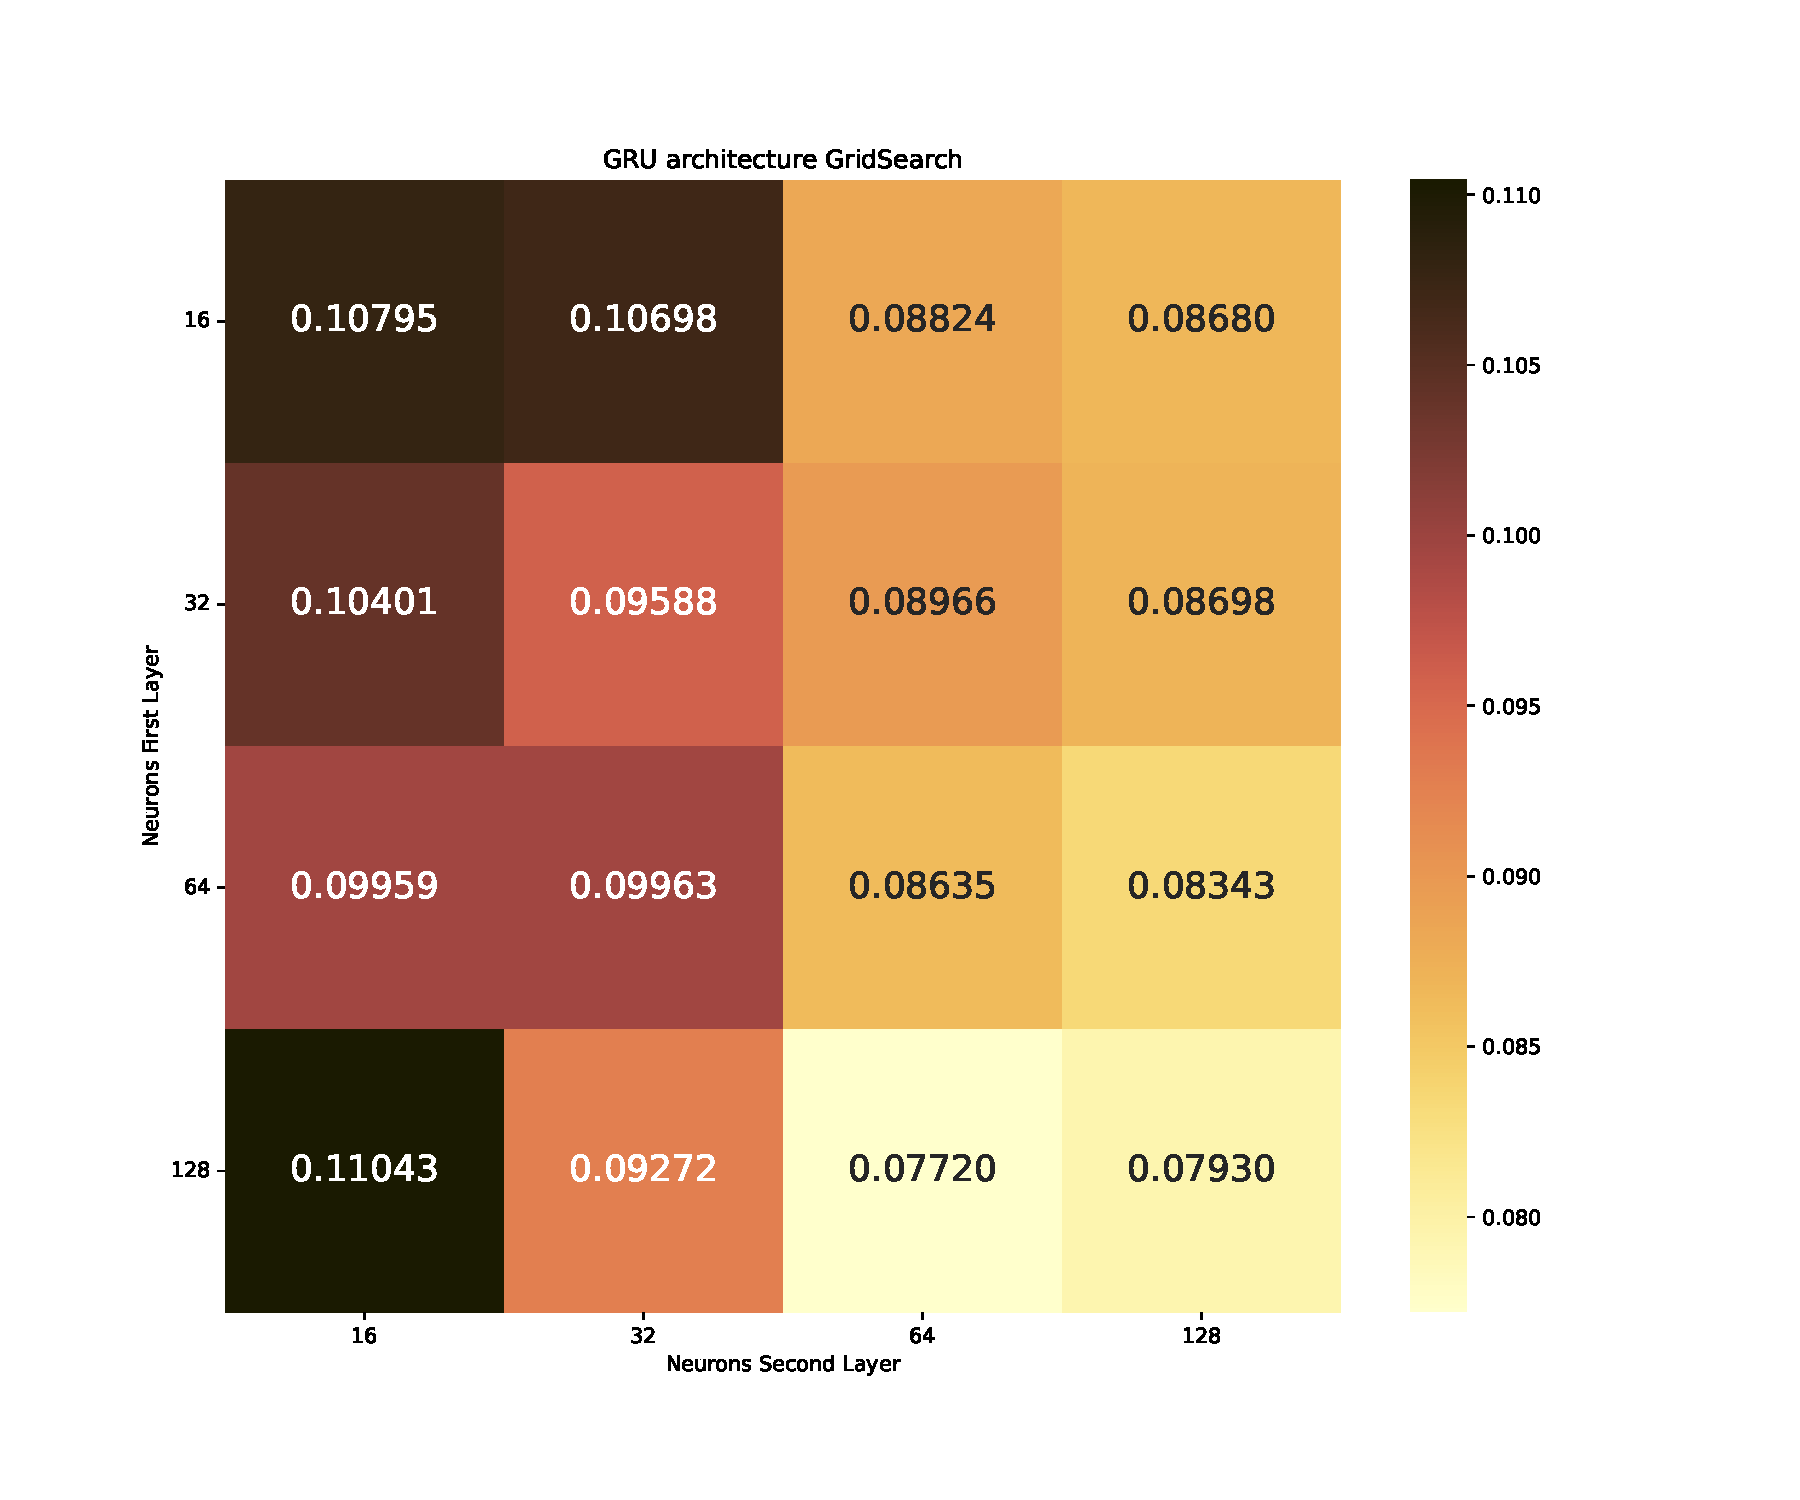
\includegraphics[width=\columnwidth]{figures/Large_forecast_gridsearch_gru.pdf}
  \caption{\label{fig_largegs}Grid Search over different combination of layer size for a multilayered multivariate SimpleRNN and GRU network using the forecasted data}
\end{figure}

Figures (\ref{fig_largegsr}) display a Grid Search approach where Mean Squared Error is dependant on the number of neurons in each layer of a two layered Deep Recurrent Neural Network. The uppermost Figure is for the SimpleRNN cell whereas the lowermost Figure is for the GRU cell. 

\subsubsection{Data alteration for long sequences}
In the context of our data, we refer to a long sequence as a input width of 168 hours, i.e. one week of data. We set up an RNN with with two GRU cells each with 128 neurons, as an immediate response to the MSE values obtained in previous results. We then performed different experiments by tweaking individual aspects of the RNN while keeping the other constant. All results for this subsection are also made using a Sequence to Sequence model, as for the results in the subsection above.

\begin{figure}
  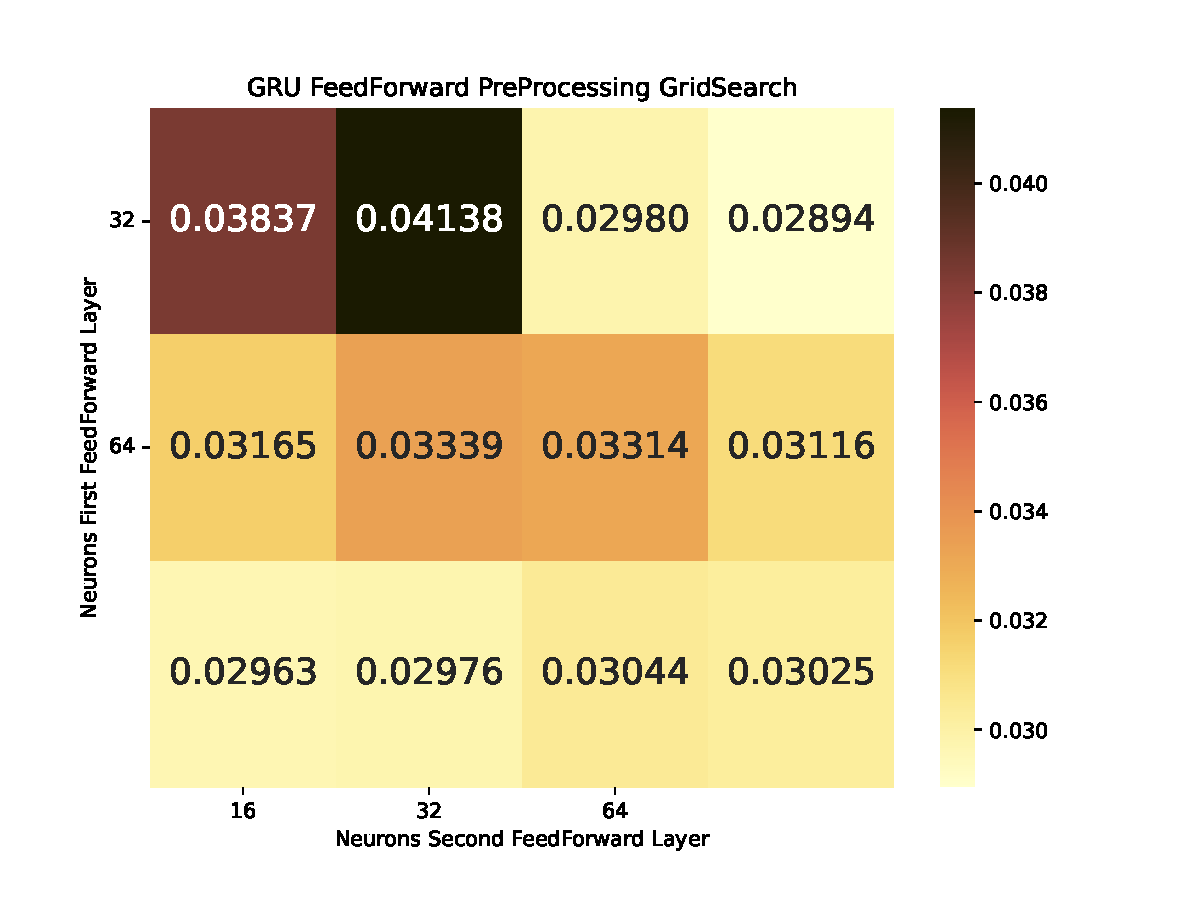
\includegraphics[width=\columnwidth]{figures/Large_forecast_ff_gridsearch_gru.pdf}
  \caption{\label{fig_gsff}Grid search over different architectures utilizing Dense layers preceding the GRU layers}
\end{figure}

Figure (\ref{fig_gsff}) displays a Grid Search performed over different architectures where one or two Dense Feed Forward layers preceded the GRU layers in the RNN.

\begin{figure}
  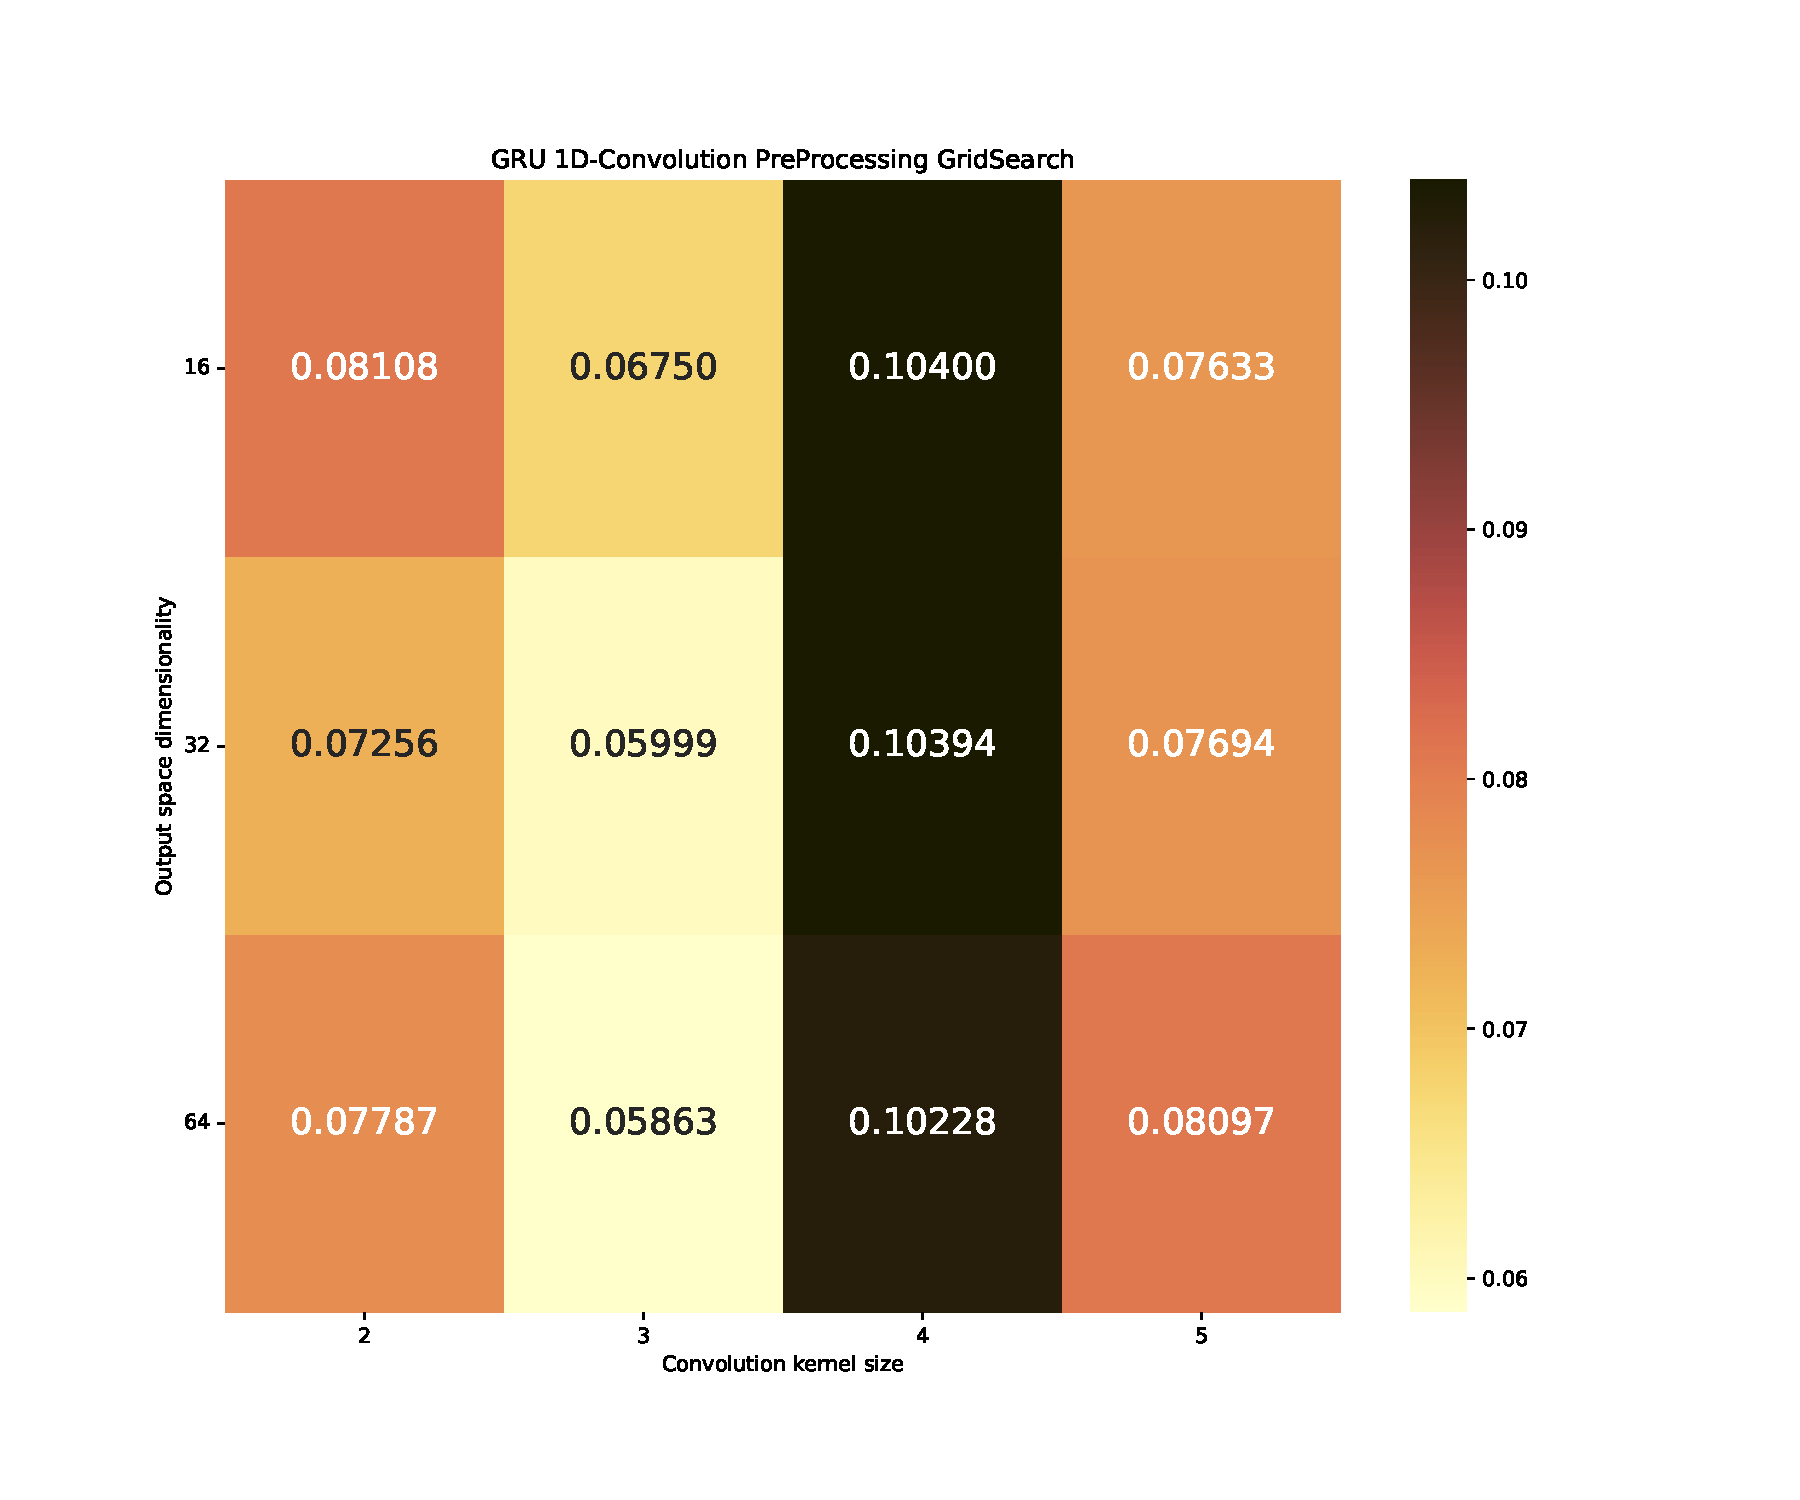
\includegraphics[width=\columnwidth]{figures/Large_forecast_conv_gridsearch_gru.pdf}
  \caption{\label{fig_gsconv}Grid Search over different architectures utilizing a 1 Dimensional convolutional layer preceding the GRU layers}
\end{figure}

Figure (\ref{fig_gsconv}) shows a Grid Search performed over different output space dimensionality and kernel sizes, with a fixed stride of 3.

\begin{figure}
  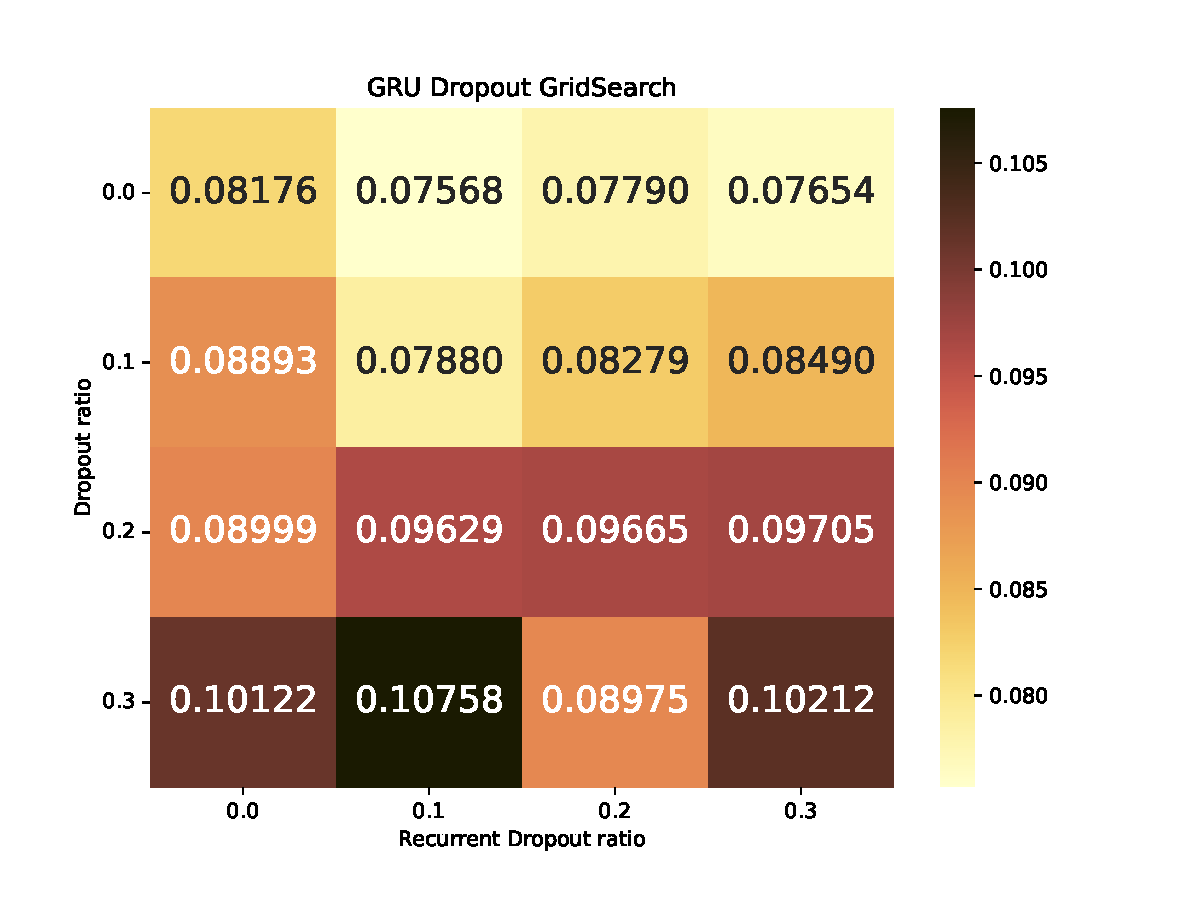
\includegraphics[width=\columnwidth]{figures/Large_forecast_dropout_gridsearch_gru.pdf}
  \caption{\label{fig_gsdrop}Grid Search over different ratios of dropout and recurrent dropout.}
\end{figure}

Finally, Figure (\ref{fig_gsdrop}) presents a Grid Search performed over different combinations of dropout and recurrent dropout. 


\section{Discussion}

\subsection{Recurrent Neural Networks}


\subsubsection{Response to architectural changes}
As stated in the Introduction, we have developed a Recurrent Neural Network to study time-series data. For this, we have utilized the frontend Keras in conjunction with the Machine Learning library TensorFlow. In this section, we will limit ourselves to the study of our Sequence to Sequence model approach, which predicts 24 hours into the future at every time step instead of at just the final time step. This increases the number of error gradients propagated backwards through our model \cite{Geron2019}. Furthermore, for the multivariate case, we will only study the model behavior with the forecasted values in the dataset. 

By inspecting Figure (\ref{fig_smallgs}), it can be seen how the MSE varies as a function of number of neurons for a single layered, univariate model with price as its only feature. By following the curve for the SimpleRNN, as the number of neurons in the layer increases, the lower the MSE becomes. As the MSE is a negatively oriented score, this is a favorable response. However, it can be argued that both the GRU and LSTM models respond somewhat less uniform to the change in model complexity, especially for the univariate case. Moreover, though all three cells performs somewhat equal, the SimpleRNN cell attains the lowest MSE score with the highest number of neurons, i.e. 128 for the univariate case. This may be reasonable as this is for a univariate model, where the amount of data is sufficient for an SimpleRNN cell to fit the data appropriately, whereas the more complex cell structures of LSTM and GRU internally may overcomplicate the data. 

Furthermore, by moving downwards in Figure (\ref{fig_smallgs}), some similarities may be drawn between the overall behavior. However, both the SimpleRNN and GRU models are initially having a harder time fitting to the data than the LSTM cell model. As such, by introducing two more features to be used when predicting the price, the SimpleRNN may be overloaded with data such that it is having a harder time extracting the relevant structures for further predictions. However, this may not be the case for the LSTM cell network, where it seems that the internal gates are able to extract and remember the relevant structures even with a lower neuron count. Interestingly, the LSTM network performs better with the multivariate data than the univariate data for already at 32 neurons. Thus, the two plots in Figure (\ref{fig_smallgs}) may indicate that the SimpleRNN is sufficient for univariate data, while for the multivariate case it is more suitable to use an LSTM or GRU. This may be a consequence of the short-term memory problem of SimpleRNN cells, as the multivariate feature space is three times as large as the univariate feature space. Thus, having a long-term memory component as found in the LSTM and GRU cell is necessary to not discard relevant information during training.

Figure (\ref{fig_largegs}) are Grid Search approaches to determine how the Mean Squared Error responds to a change in architecture for a two layered dense multivariate model. Inspecting the uppermost Figure in (\ref{fig_largegs}), it can be seen that the MSE responds somewhat similarly to the multilayered model as for the single layered SimpleRNN model. Namely that the MSE attains lower values as the complexity of both layers are increased, though that the MSE is relatively high for less complex architectures. This trend is similar for the lowermost Figure in (\ref{fig_largegs}), which displays the same Grid Search but for a GRU model instead. It can argued that the lowest MSE is attained with the most complex model, as there seem to be a relationship between MSE value and second layer complexity, with higher second layer complexity being better. However, the best result is attained for 128 and 32 neurons as seen in the Figure, though this may be a stochastic result which arises from the weight initialization of the modes. We note that the results are not entirely consistent between model compilations (not shown), though the relationship between the MSE and model complexity as shown in Figures (\ref{fig_smallgs}) and (\ref{fig_largegs}) is consistent between model runs. 

\subsubsection{Effect of data alteration for long sequences}
It has been noted in previous sections that there are two central drawbacks for Recurrent Neural Networks, namely the gradient problem and the short-term memory problem, especially for long sequences of data \cite{Geron2019}. As a measure to decrease the effects of these limitations, we have tried several preprocessing layers as well as studied the effect of Dropout. For preprocessing layers, we have studied the effect of preprocessing the data using one or two Dense FeedForward layers before the Recurrent Network layers, with the intent that the FeedForward layers may project our data into a more suitable feature space before being fed to the Recurrent Neural Network. The result of preprocessing the data with one or two FeedForward Dense layers can be seen in Figure (\ref{fig_gsff}). For clarity, all results in this section has been produced using a Sequence-to-Sequence multivariate GRU following the optimal architecture as argued for by combining the results of Figure (\ref{fig_smallgs}) and (\ref{fig_largegs}), i.e. two Recurrent layers both with 128 neurons each.

By inspecting Figure (\ref{fig_gsff}), there seem to be no clear pattern in how the MSE is affected by different FeedForward architectures. Though some architectural combinations do achieve a somewhat equal MSE to the model with no preprocessing layers at all, the results do seem to be consistently worse across all combinations of Dense layer architecture.  

Figure (\ref{fig_gsconv}) shows a Grid Search approach which studies the implementing of a 1-dimensional convolutional layers which precedes the two Recurrent layers. The 1-dimensional layer downsamples the input sequence, as well as preserving the notable structures in the data through convolution \cite{Geron2019}. This process helps the coming Recurrent layers to detect larger patterns in the data, by making the sequences to detect shorter. As can be seen in Figure (\ref{fig_gsconv}), the effect of the 1-dimensional convolutional layer seem to be somewhat tied to the size of the convolutional kernel, more so than the number of output features of the layer. Though the distribution shown in Figure (\ref{fig_gsconv}) is relatively stochastic. With a kernel size of three, the model attains lower MSE values than what was reported in figure (\ref{fig_largegs}). As such, a 168-hour input width may prove longer than what the short-term memory of a Recurrent Neural Network is able to retain, as the MSE attains a better score with downsampled data for some combinations of output space dimensionality and kernel size. However, other combinations do deter the overall MSE score, such that there is no clear benefit of applying the convolutional layer unless the parameters are tuned to fit the current data.

Finally, the effect of Dropout and Recurrent Dropout can be seen in Figure (\ref{fig_gsdrop}). The central idea behind dropout is to generalize the training data by deactivating a ratio of the current neurons, i.e. setting their internal value to 0 essentially stopping all incoming signals. By inspecting Figure (\ref{fig_gsdrop}), a single MSE value, that being the rightmost uppermost corner value related to Dropout = 0 and Recurrent Dropout = 0.3 do achieve a lower MSE value than what was reported in Figure (\ref{fig_largegs}). However, the trend is that Dropout heightens the MSE value, with regular Dropout having a more severe negative impact to the MSE than Recurrent Dropout. This may be due to the training sample used being relative sparse, only counting a total of $\tilde1500$ individual samples. As such, the dropout removes important information from the dataset, which may not be covered elsewhere, instead of generalizing the dataset. 

\subsection{Recurrent Neural Network}

\section{Conclusions}

\appendix

\section{Source Code}
\label{sec:sc}
Link to github repository containing all developed code for this project: \textbf{CORRECT URL HERE}%\url{https://github.com/AndreasBordvik/FYS-STK4155-Prj2_report}

% Create the reference section using BibTeX:

% ------------------- end of main content ---------------

\bibliographystyle{plain}
\bibliography{biblio}




\end{document}

